\chapter{Appendix}
\label{cha:appendix}

\section{Additional Health Information}

This section defines the different diseases that the patients in our study were recorded as having, but it was not known who had which. This lack of detailed information prevents further classification within our dataset, but highlights potential areas for future research.

\subsection{Hypertrophic Cardiomyopathy}

Hypertrophic cardiomyopathy (HCM) is the most prevalent genetic cardiovascular disorder in the United States, affecting approximately one in every 500 individuals. A minority of those diagnosed with HCM experience severe complications, such as end-stage heart failure necessitating a transplant, cardiovascular mortality, including deaths from heart failure, and sudden cardiac death. Current risk stratification methods rely on a few predictors like family history of sudden death, syncope (temporary loss of consciousness due to a drop in blood pressure), and non-sustained ventricular tachycardia (short episodes of fast heart rhythms originating from the ventricles). These methods often fall short in accurately predicting adverse outcomes, especially for patients at intermediate risk who might not display conventional risk factors. This lack of precise predictive tools has hindered the identification of high-risk individuals who could benefit from more frequent monitoring and aggressive management of symptoms ~\cite{KOCHAV2021117}.

ML models have shown promise in enhancing risk prediction across various cardiovascular conditions. These models surpass traditional logistic or linear regression approaches by considering complex, non-linear interactions among predictors, leading to more reliable forecasts. In the realm of HCM, there have been attempts to use data-driven models to assess the risk of ventricular arrhythmias (abnormal heart rhythms originating from the lower chambers of the heart), though these retrospective studies have typically shown low specificity (the ability to correctly identify those without the condition). Recent advancements have included the development of a convolutional neural network (a type of deep learning model that is particularly effective for analyzing visual data) that successfully diagnoses HCM using only electrocardiogram data. Despite these developments, predicting severe cardiac incidents remains challenging due to the absence of robust prediction models. This prospective cohort study aims to enhance the prediction of adverse cardiac events in HCM patients using advanced ML models ~\cite{KOCHAV2021117}.

\subsection{Amyloidosis}


Cardiac amyloidosis is an uncommon but serious form of restrictive cardiomyopathy characterized by the uncontrolled deposition of amyloid proteins, which impairs organ function. This disease is often underdiagnosed because its clinical manifestations resemble those of more prevalent hypertrophic conditions. Accurately diagnosing cardiac amyloidosis early is essential for initiating effective treatment, but the diagnosis is commonly delayed because its symptoms can easily be confused with those of other cardiac diseases ~\cite{ijms24065680}.

There are various types of cardiac amyloidosis, each classified according to the specific proteins that form the amyloid deposits. Differentiating among these types is crucial because each type requires a distinct therapeutic approach. The diagnostic process typically involves identifying certain clinical signs, alongside electrocardiographic and imaging findings suggestive of amyloidosis. Confirmation usually requires histological evidence of amyloid presence (examining tissue samples under a microscope to identify amyloid deposits), which can complicate the diagnosis further ~\cite{ijms24065680}.

Emerging technologies with the help of ML and AI are being explored to overcome these diagnostic challenges. These technologies have the potential to automatically extract significant information from clinical data, bypassing the need for the extensive preprocessing typically required in traditional diagnostic approaches. This review discusses the potential of these advanced computational techniques to improve the accuracy and timeliness of cardiac amyloidosis diagnosis, potentially leading to better patient outcomes by allowing for earlier and more targeted treatment strategies ~\cite{ijms24065680}.

\subsection{Cushing's Syndrome}

Cushing's syndrome (CS) is a disorder caused by prolonged exposure to high levels of cortisol, leading to symptoms such as weight gain, high blood pressure, and changes in skin appearance. The accurate classification of CS is critical for early diagnosis, facilitating timely treatment and improving patient outcomes. Diagnosing CS is complex and requires the interpretation of clinical signs, biochemical test results, and medical imaging by specialized physicians. The work of ~\textcite{CS} explores advanced ML algorithms to aid as clinical decision support systems in diagnosing, prognosis, and treating CS. It evaluates several algorithms, with the RF algorithm proving most effective, demonstrating an average accuracy of 92$\%$ and an f1-score of 91.5$\%$. The RF-based models, particularly the one vs. all binary classification, showed high sensitivity (97.6$\%$), precision (91.1$\%$), and specificity (87.1$\%$) in distinguishing CS from non-CS cases. Moreover, the multiclass model effectively categorized different CS subtypes with high accuracy.

Early and accurate diagnosis is challenging due to symptom overlap with common conditions and inconsistent test results influenced by various factors. The study of ~\textcite{CS} supports the use of ML to enhance diagnostic processes. They have developed a publicly accessible web application that provides CS predictions based on patient test results. This tool and the underlying models, developed using the Python scikit-learn library, are available online for clinical and public use, aiming to support healthcare professionals in managing CS effectively ~\cite{CS}.

\section{Distributions}

In this section, all distributions of the sample and study datasets are listed. This should make it easier to visualize the data. Otherwise, these distributions can also be found in chapters ~\ref{cha:exampleDataset} and ~\ref{cha:studyDataSet} in the cross entropy.

\subsection{Distributions of the Example Dataset}

Especially the distributions of heart rates (blue distribution) are important insofar as they allow us to directly observe commonalities and peculiarities. In the case of the younger female subject, it is evident that her pulse is higher both at rest and during activity, which can be attributed to her age. For the older subject, the distribution resembles a Gamma distribution. In contrast, the younger female subject presents an additional peculiarity. Firstly, her distribution does not fit any known mathematical distribution, and secondly, there is a notably high number of elevated pulse rates within the distribution. This suggests that the individual is either very physically active or tends to have a high pulse rate with minimal exertion.

\FloatBarrier
\begin{figure}[h!]
  \centering
  \begin{minipage}[b]{0.7\linewidth}
    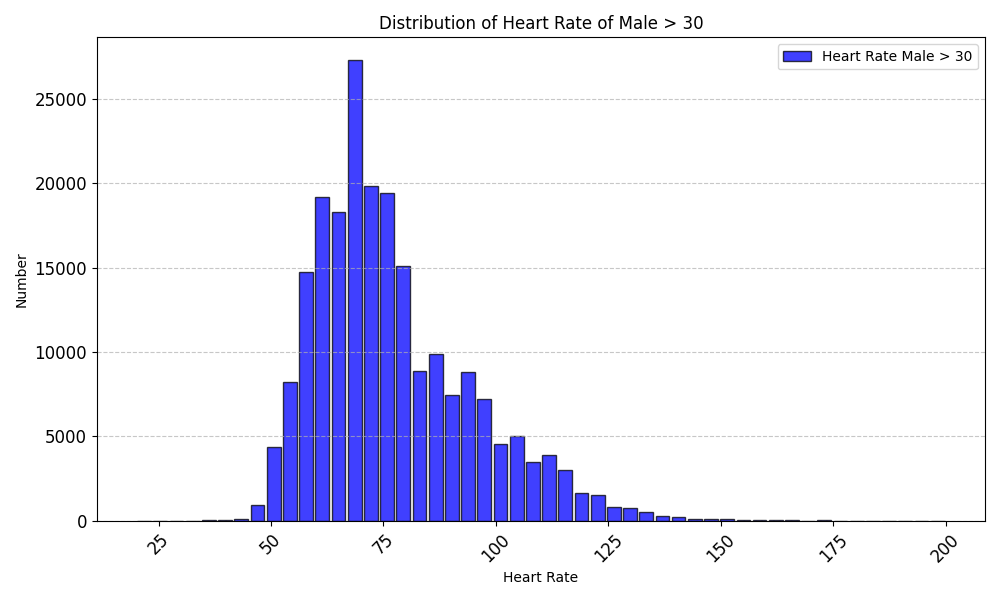
\includegraphics[width=\linewidth]{Master Thesis/Plots/Dist_HeartRate.png}
    \caption{Heart rate distribution in a male subject over 30 years of age}
    \label{fig:DistHeartMichi}
  \end{minipage}
  \quad % Fügt etwas Platz zwischen den Bildern ein
  \begin{minipage}[b]{0.7\linewidth}
    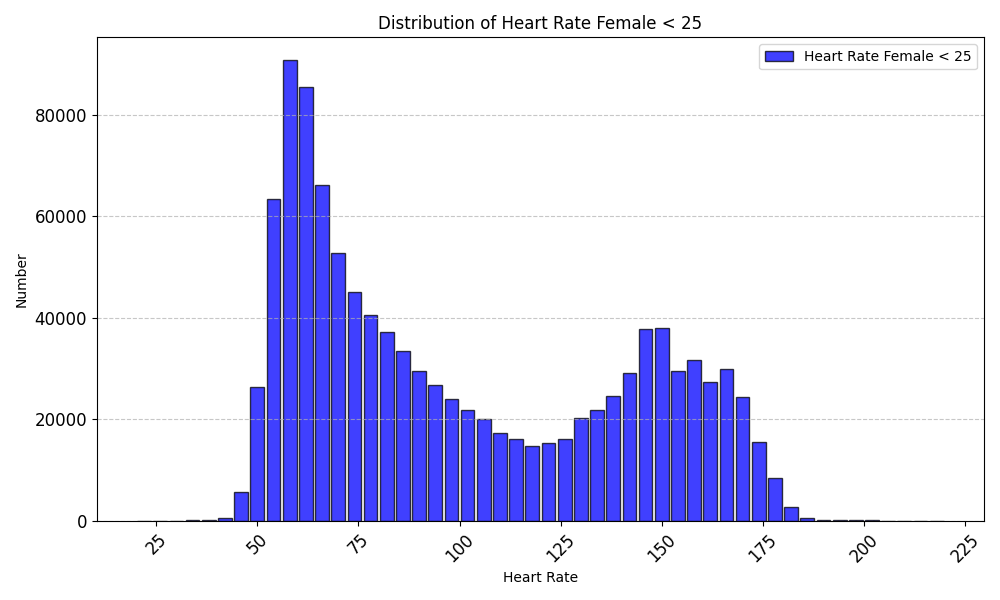
\includegraphics[width=\linewidth]{Master Thesis/Plots/Dist_HeartRate_Tanja.png}
    \caption{Heart rate distribution in a female test subject under 25 years of age}
    \label{fig:DistHeartTanja}
  \end{minipage}
\end{figure}
\FloatBarrier

However, it is not only the distribution of the heart rate that is interesting to take a closer look at here, but also that of the calories burned in activity. 

\FloatBarrier
\begin{figure}[h!]
  \centering
  \begin{minipage}[b]{0.7\linewidth}
    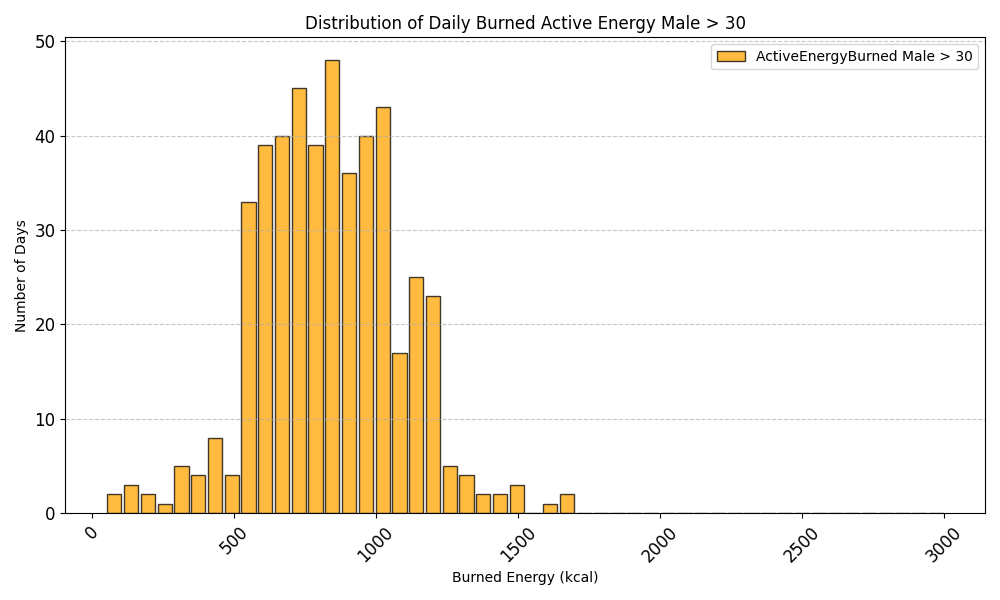
\includegraphics[width=\linewidth]{Master Thesis/Plots/Dist_ActiveEnergyBurned.png}
    \caption{Distribution of burned energy in action of a male subject over 30 years of age}
    \label{fig:ValuesMichiactive}
  \end{minipage}
  \quad % Fügt etwas Platz zwischen den Bildern ein
  \begin{minipage}[b]{0.7\linewidth}
    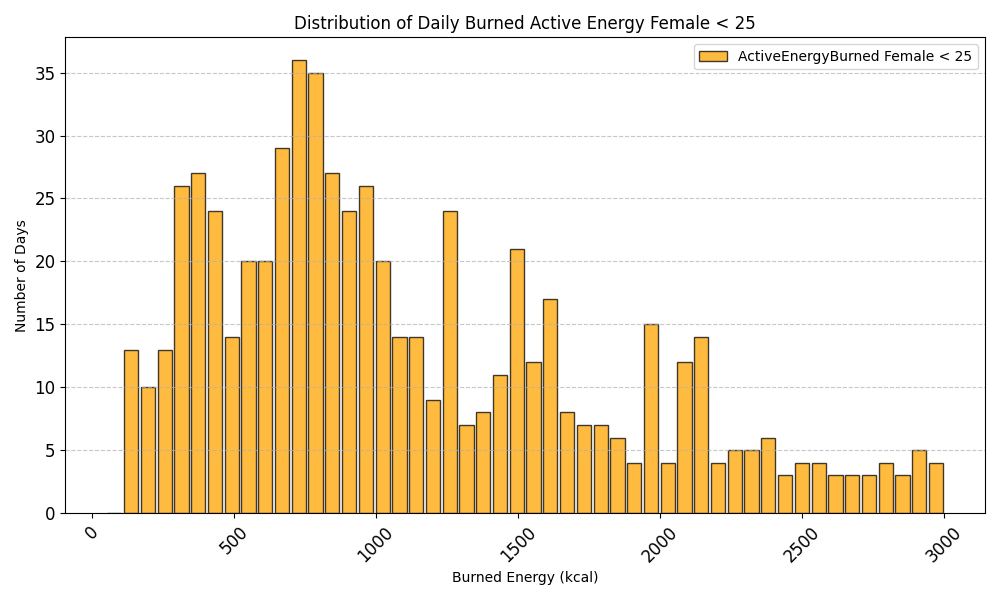
\includegraphics[width=\linewidth]{Master Thesis/Plots/Dist_ActiveEnergyBurned_Tanja.png}
    \caption{Distribution of burned energy in action of a female test subject under 25 years of age all relevant values}
    \label{fig:ValuesTanjaactive}
  \end{minipage}
\end{figure}
\FloatBarrier

If we only look at the distribution, we see that the male test subject recorded fewer extremely low values (under 500 calories) and also few extremely high values (over 1200 calories). Mostly we are between 500 calories and 1000 calories. This indicates above all that this test person is definitely exercising regularly.
In the female test subject, on the other hand, we have a very wide spread of frequency and a large variance in calories burned in activity. We also see some frequencies above 2000 calories. This suggests that the subject recorded some sessions that lasted several hours or recorded several sessions per day.

The distribution of calories burned in general is also interesting. Here we see large differences between the test subjects. 
\FloatBarrier
\begin{figure}[h!]
  \centering
  \begin{minipage}[b]{0.45\linewidth}
    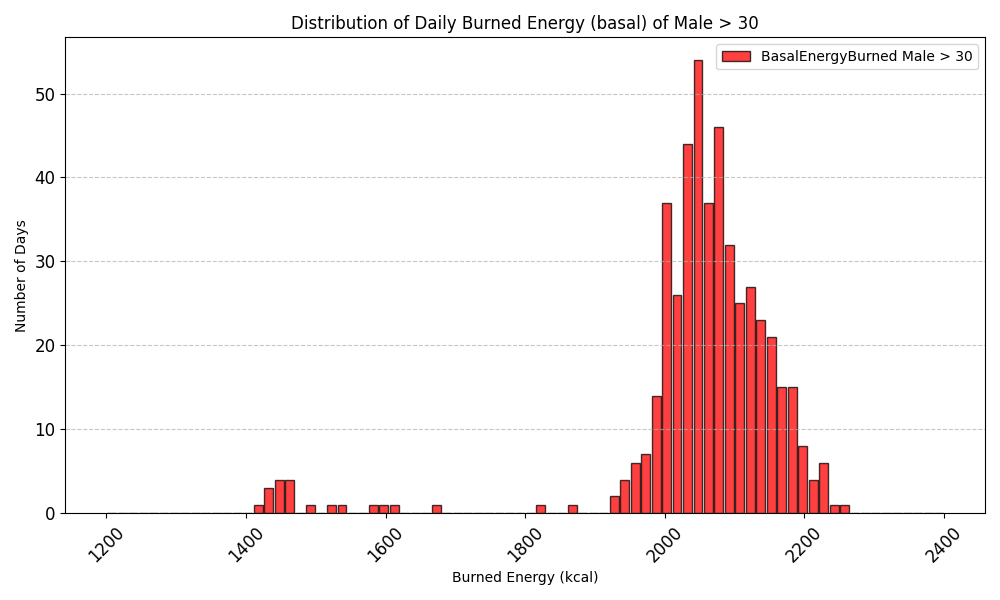
\includegraphics[width=\linewidth]{Master Thesis/Plots/Dist_BasalEnergyBurned.png}
    \caption{Distribution of burned energy in overall of a male subject over 30 years of age all relevant values}
    \label{fig:ValuesMichibasal}
  \end{minipage}
  \quad % Fügt etwas Platz zwischen den Bildern ein
  \begin{minipage}[b]{0.45\linewidth}
    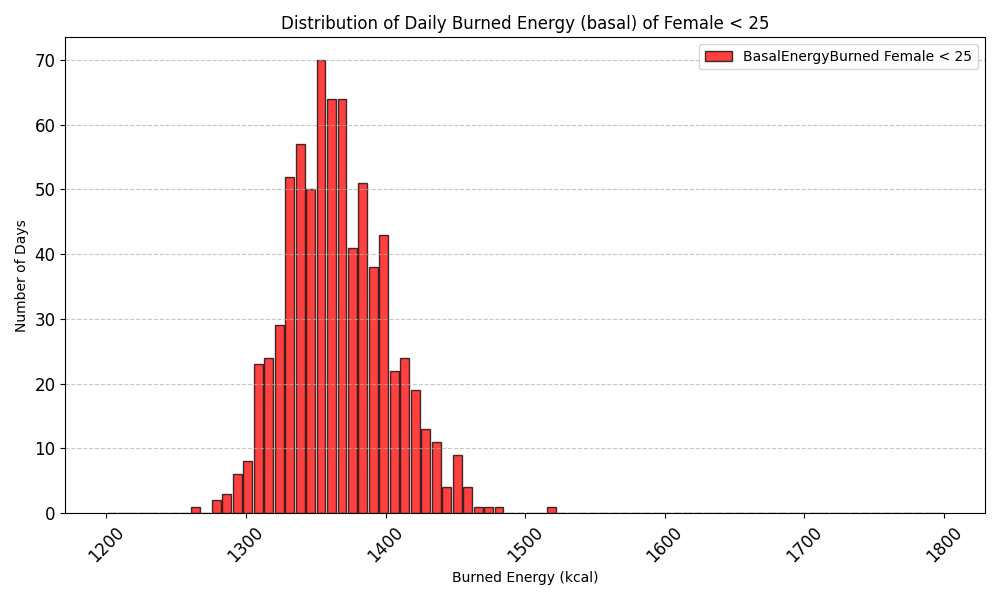
\includegraphics[width=\linewidth]{Master Thesis/Plots/Dist_BasalEnergyBurned_Tanja.png}
    \caption{Distribution of burned energy in overall of a female test subject under 25 years of age all relevant values}
    \label{fig:ValuesTanjabasal}
  \end{minipage}
\end{figure}
\FloatBarrier

In any case, we can clearly see here that the total number of calories consumed by the male test subject is higher on average than that of the female test subject. On the one hand, this is actually due to the respective biological sex, but also in any case to the type of activity. For example, the body still burns some calories hours later after strength training, whereas the body burns a lot of calories during fitness training but not as many afterwards. What is surprising is that the female test subject's calories appear very low compared to the calories burned during the activity. Of course, this could be due to measurement errors, but it could also indicate that this person only does endurance sports.


To make inferences about the lifestyles of the participants, it's also interesting to examine the distribution of distances covered. This includes both walking and running distances.

\FloatBarrier
\begin{figure}[h!]
  \centering
  \begin{minipage}[b]{0.7\linewidth}
    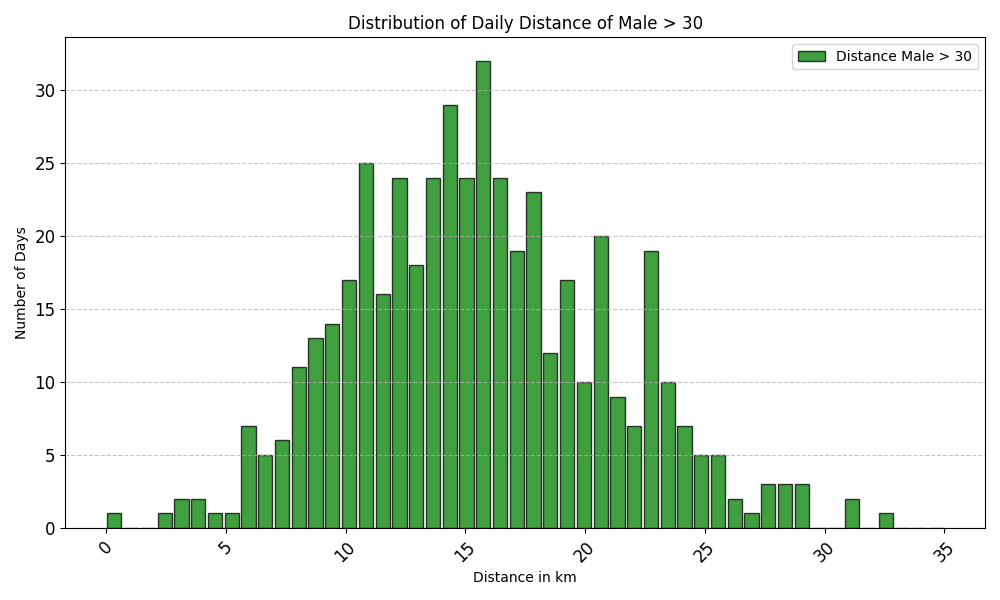
\includegraphics[width=\linewidth]{Master Thesis/Plots/Dist_DailyDistance.png}
    \caption{Distribution of daily walking or running distance of a male subject over 30 years of age all relevant values}
    \label{fig:ValuesMichiwalk}
  \end{minipage}
  \quad % Fügt etwas Platz zwischen den Bildern ein
  \begin{minipage}[b]{0.7\linewidth}
    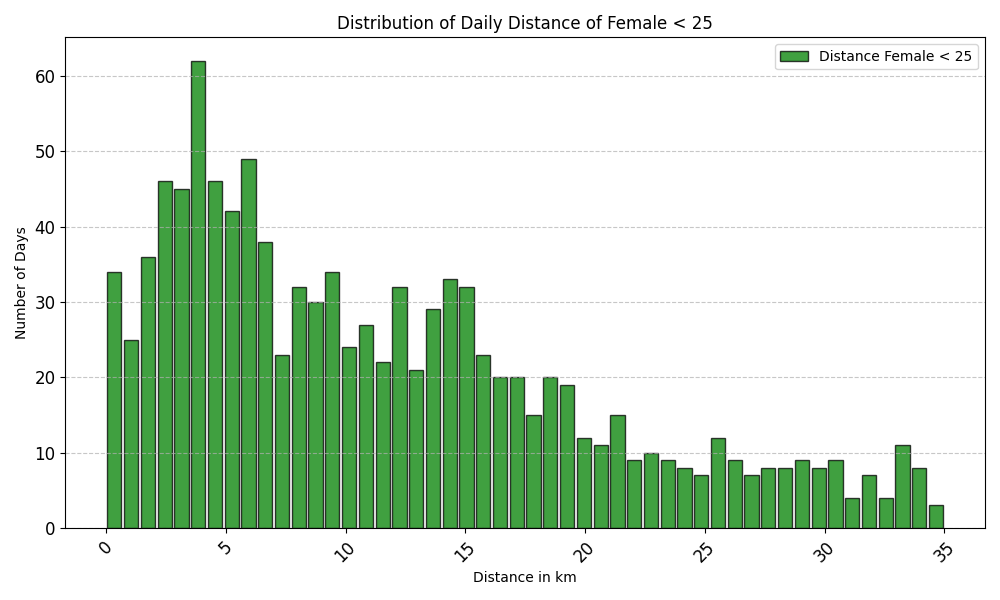
\includegraphics[width=\linewidth]{Master Thesis/Plots/Dist_DailyDistance_Tanja.png}
    \caption{Distribution of daily walking or running distance of a female test subject under 25 years of age all relevant values}
    \label{fig:ValuesTanjawalk}
  \end{minipage}
\end{figure}
\FloatBarrier

We see here that the male subject seems to move very regularly. It appears he almost always covers the WHO-recommended distance of about 8 km. He often goes much further and seems to jog frequently to reach over 18 km. He rarely covers more than 25 km. For the female subject, we observe that she often does not cover the recommended daily distance. Her highest frequencies are between 0 and 5 km. Unlike the male participant, we see she does cover some very long distances at times, even over 30 km, which might suggest there are days when she hardly moves at all to ensure rest days and allow her body enough recovery.

\subsection{Distributions of the Study Dataset}

The following visualizations provide valuable insights into the differences and similarities in various health metrics between male and female subjects within the study dataset. Each color is used to represent a specific metric: blue for heart rates, orange for active energy burned, red for basal energy burned, and green for walked distance. This color-coded categorization facilitates a clear and straightforward comparison of these metrics between sex, highlighting the unique patterns and trends observed in the data.

\FloatBarrier
\begin{figure}[h!]
  \centering
  \begin{minipage}[b]{0.7\linewidth}
    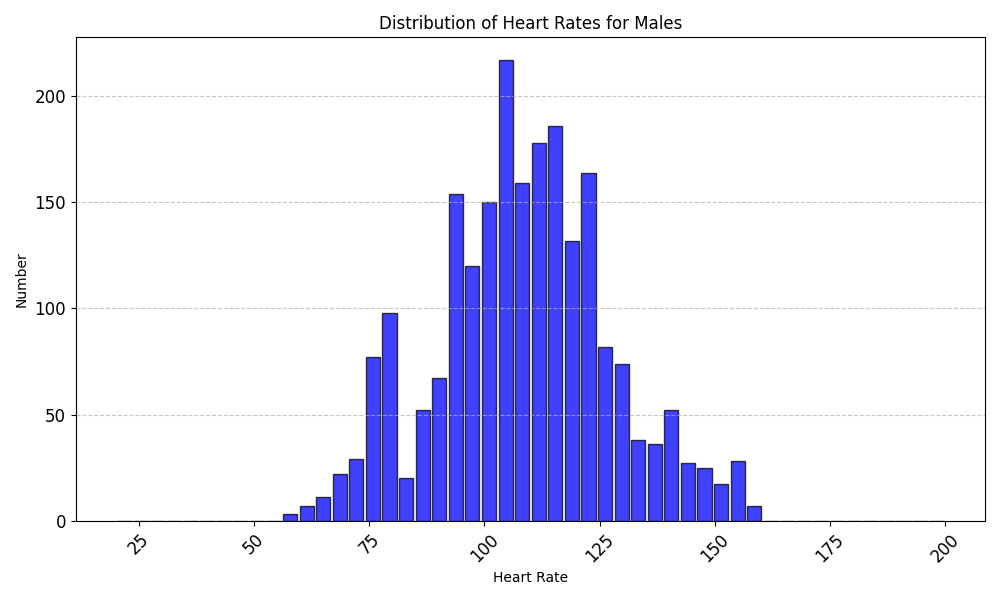
\includegraphics[width=\linewidth]{Master Thesis/Plots/Dist_HeartRate_Males.png}
    \caption{Heart rate distribution of all male subjects}
    \label{fig:subjmaleheart}
  \end{minipage}%
  \quad
  \begin{minipage}[b]{0.7\linewidth}
    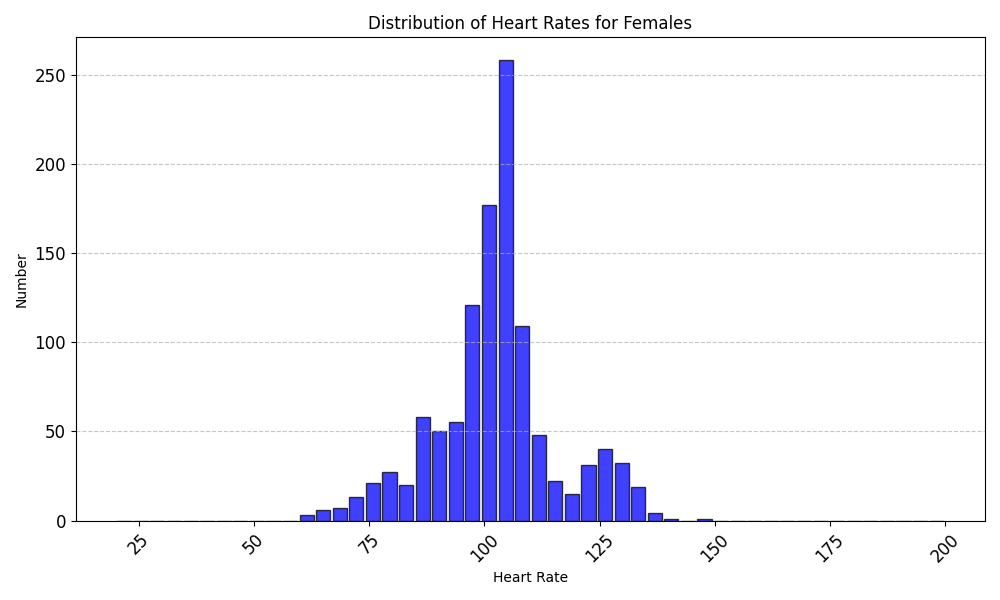
\includegraphics[width=\linewidth]{Master Thesis/Plots/Dist_HeartRate_Females.png}
    \caption{Heart rate distribution of all female subjects}
    \label{fig:subjfemaleheart}
  \end{minipage}
\end{figure}
\FloatBarrier

This image ~\ref{fig:subjmaleheart} shows the distribution of heart rates for males, depicted in blue. The histogram illustrates a central tendency with the majority of heart rates clustering around the middle values, indicating a normal distribution with some variation. In contrast, image ~\ref{fig:subjfemaleheart} displays the heart rate distribution for females, also in blue. Similar to the males, there is a noticeable peak indicating the most common heart rate range, but with a slightly different spread and central tendency.

\FloatBarrier
\begin{figure}[h!]
  \centering
  \begin{minipage}[b]{0.7\linewidth}
    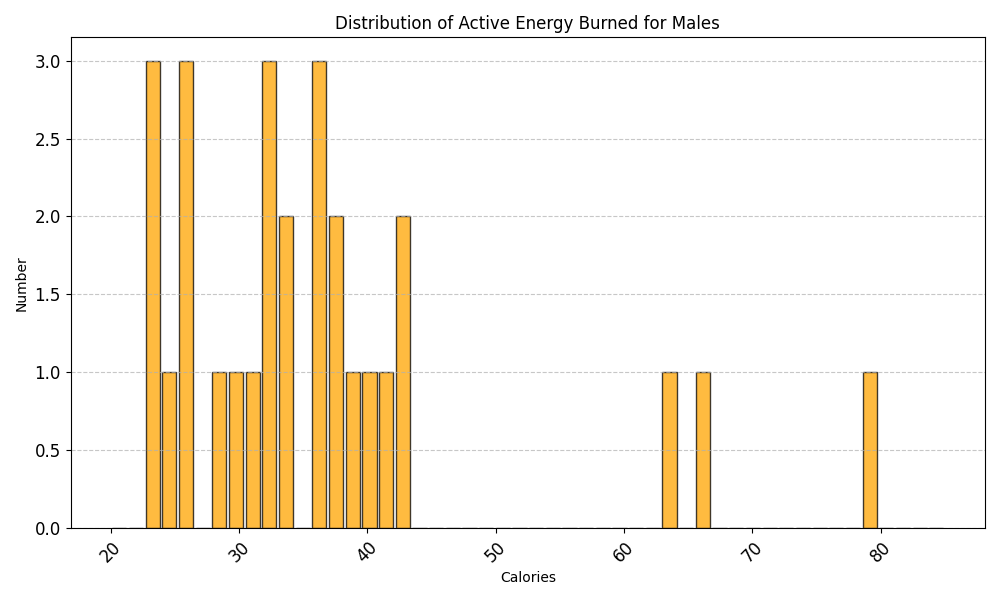
\includegraphics[width=\linewidth]{Master Thesis/Plots/Dist_ActiveEnergy_Males.png}
    \caption{Distribution of burned energy in action of all male subjects}
    \label{fig:Valuesactiveallmale}
  \end{minipage}%
  \quad
  \begin{minipage}[b]{0.7\linewidth}
    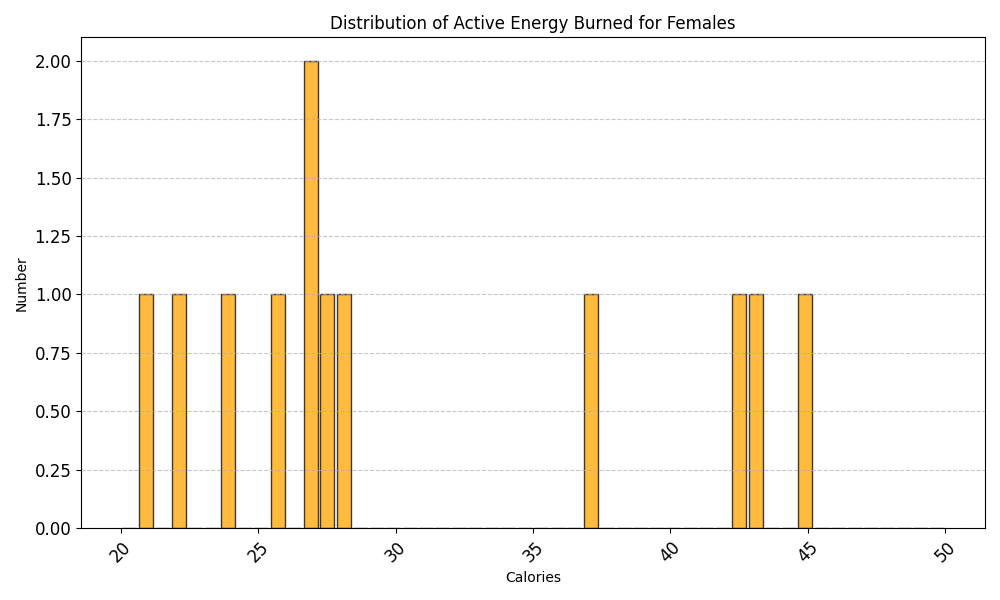
\includegraphics[width=\linewidth]{Master Thesis/Plots/Dist_ActiveEnergy_Females.png}
    \caption{Distribution of burned energy in action of all female subjects}
    \label{fig:Valuesactiveallfemale}
  \end{minipage}
\end{figure}
\FloatBarrier

In the second image, the distribution of active energy burned is shown in orange. Image ~\ref{fig:Valuesactiveallmale} represents the data for males, which appears more spread out with several peaks, indicating varied levels of energy expenditure among the male subjects. Image ~\ref{fig:Valuesactiveallfemale} shows the distribution for females, featuring a different pattern of energy expenditure. There are fewer peaks and a distinct concentration of values, suggesting a different pattern of activity compared to males.

\FloatBarrier
\begin{figure}[h!]
  \centering
  \begin{minipage}[b]{0.7\linewidth}
    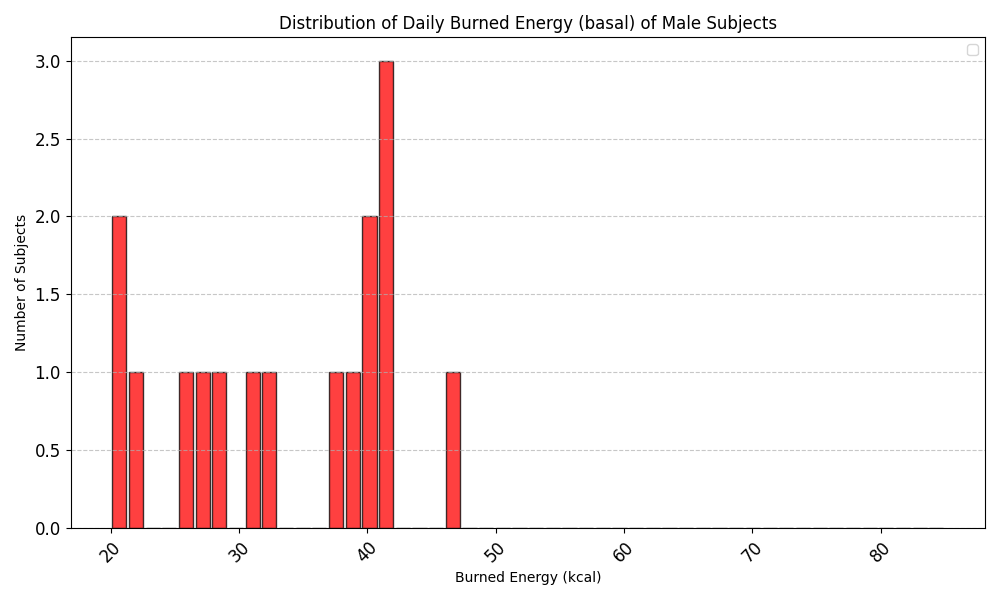
\includegraphics[width=\linewidth]{Master Thesis/Plots/Dist_BasalEnergyBurned_Male.png}
     \caption{Distribution of burned energy in overall of all male subjects}
    \label{fig:Valuesallmalebasal}
  \end{minipage}%
  \quad
  \begin{minipage}[b]{0.7\linewidth}
    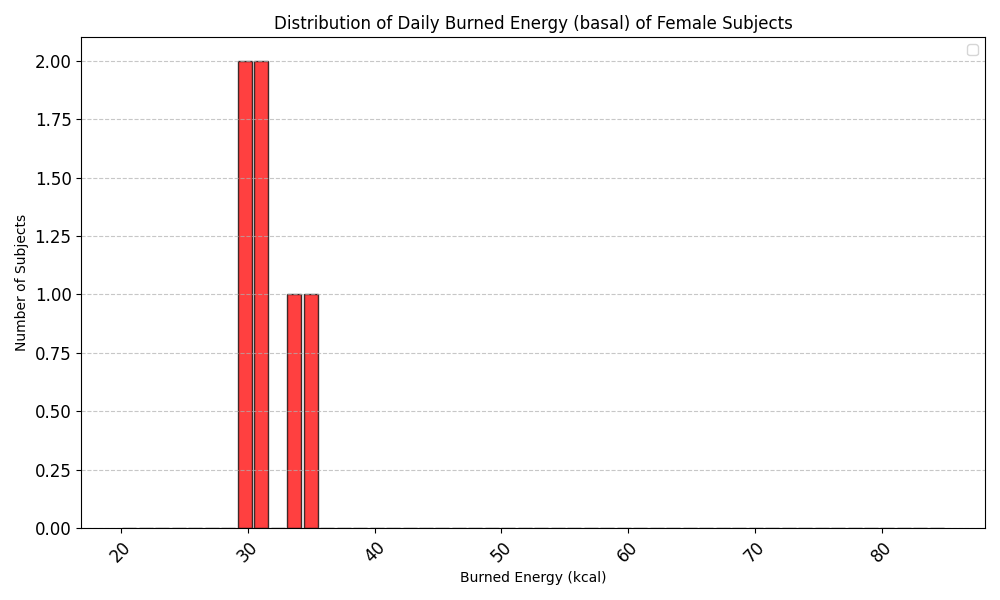
\includegraphics[width=\linewidth]{Master Thesis/Plots/Dist_BasalEnergyBurned_Female.png}
    \caption{Distribution of burned energy in overall of all female subjects}
    \label{fig:Valuesallfemalebasal}
  \end{minipage}
\end{figure}
\FloatBarrier

The third image presents the distribution of basal energy burned in red. For male subjects, shown in image ~\ref{fig:Valuesallmalebasal}, the graph highlights how energy is expended in a resting state, with a spread indicating varied metabolic rates among the males. Image ~\ref{fig:Valuesallfemalebasal} displays the distribution for female subjects, which shows a similar pattern but with a more distinct central peak, suggesting a more consistent basal metabolic rate among the females.

\FloatBarrier
\begin{figure}[h!]
  \centering
  \begin{minipage}[b]{0.7\linewidth}
    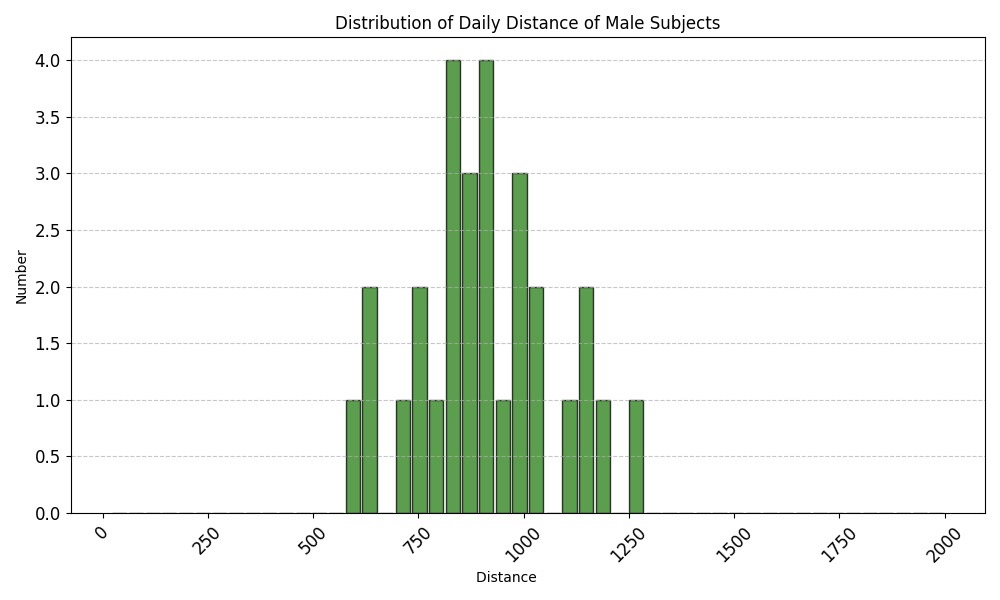
\includegraphics[width=\linewidth]{Master Thesis/Plots/Dist_Dist_Males.jpeg}
    \caption{Distribution of daily walking or running distance in meter of all male subjects}
    \label{fig:Valuesallmalewalk}
  \end{minipage}%
  \quad
  \begin{minipage}[b]{0.7\linewidth}
    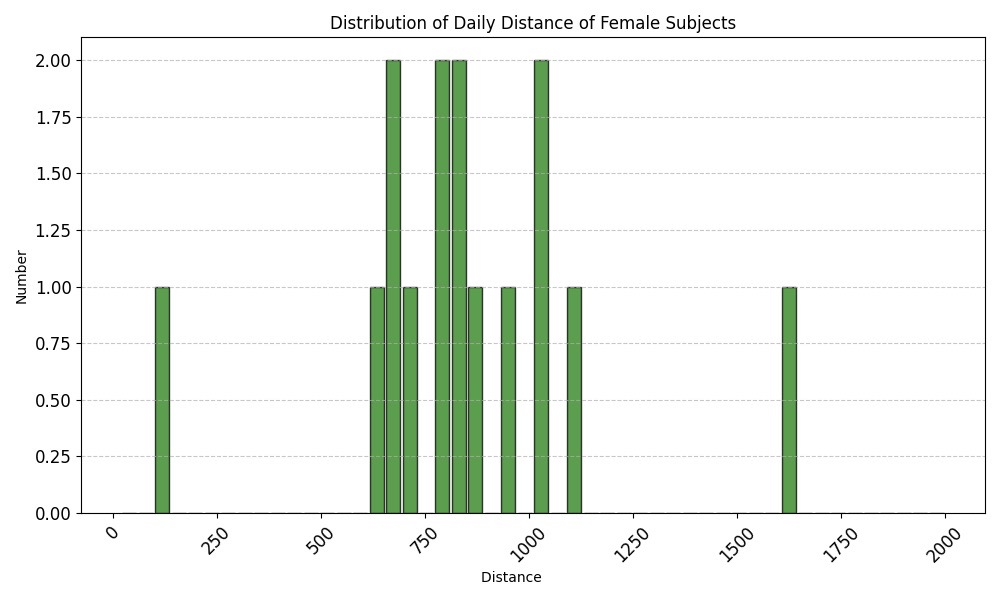
\includegraphics[width=\linewidth]{Master Thesis/Plots/Dist_Dist_Females.jpeg}
    \caption{Distribution of daily walking or running distance in meter of all female subjects}
    \label{fig:Valuesallfemalewalk}
  \end{minipage}
\end{figure}
\FloatBarrier

The fourth image illustrates the distribution of daily walked distance in meter. Image ~\ref{fig:Valuesallmalewalk} represents the daily walked distance for male subjects, indicating a central clustering with varied distances walked daily, reflecting differing levels of physical activity. In image ~\ref{fig:Valuesallfemalewalk}, the distribution for female subjects is shown, which, like the males, has a central clustering but with a noticeable difference in spread and peaks, indicating varied daily walking distances.

\section{Visual Analysis of Study Dataset}

At first, it was hard to figure out when a subject started and finished the 6MWT. So, the heart rate data was plotted to identify these times.

\FloatBarrier
\begin{figure}[h!]
  \centering
  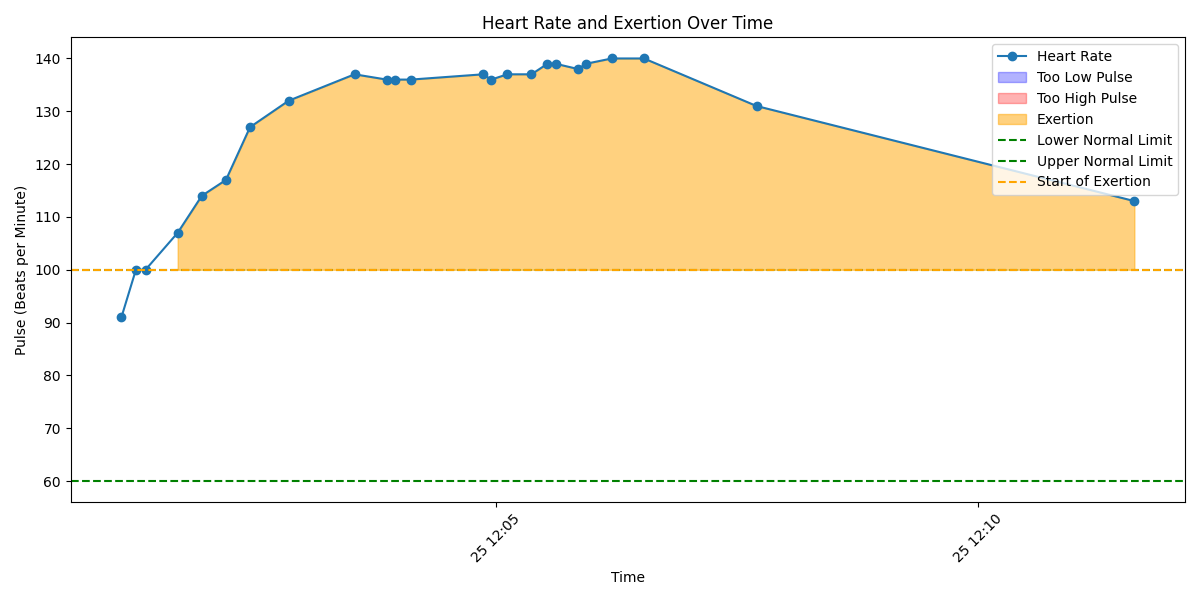
\includegraphics[width=0.8\textwidth]{Master Thesis/Plots/6MW_dataset_plot.png}
    \caption{Heart rate data plot to identify the 6MWT interval first try}
    \label{fig:6MW-study1}
\end{figure}
\FloatBarrier
The trend in the data was plotted, and a limit was determined to identify when a heart rate is 'too' high, indicating that a person is exercising.

\FloatBarrier
\begin{figure}[h!]
    \centering
    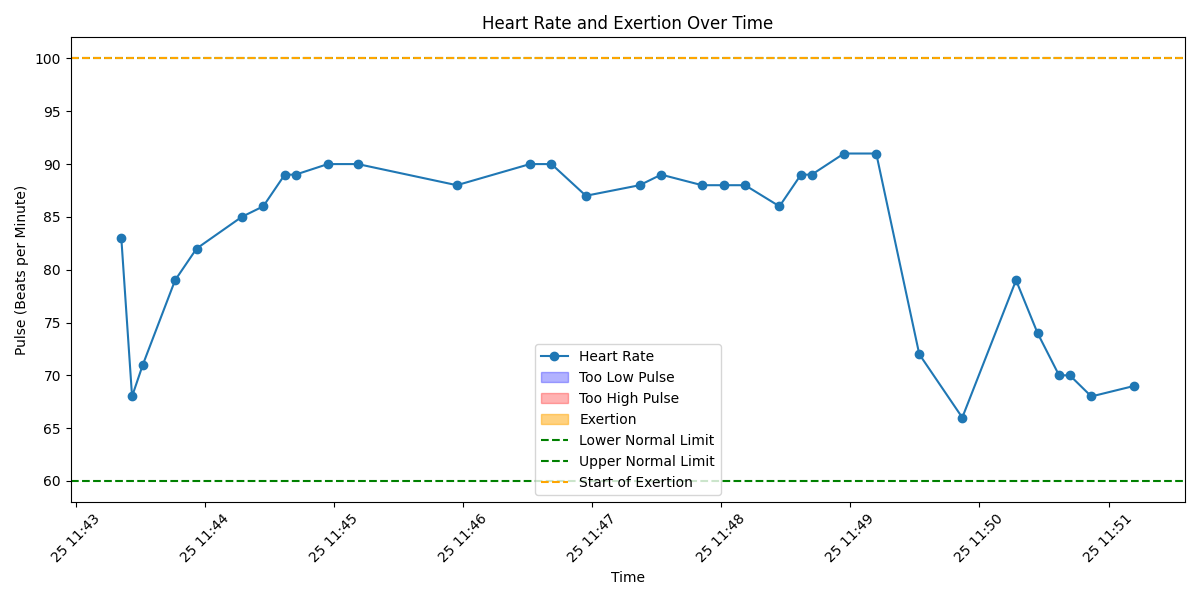
\includegraphics[width=0.8\textwidth]{Master Thesis/Plots/6MW_dataset_plot_Nr2.png}
    \caption{Heart rate data plot to identify the 6MWT interval second try}
    \label{fig:6MW-study2}
\end{figure}
\FloatBarrier

In the second figure ~\ref{fig:6MW-study2}, a potential subject was identified, and the heart rate curve was plotted. The plot seemed quite good. However, dissatisfaction with the general plot led to the decision to split everything into each day of measurement. The pictures can be seen below.

The plots above show the respective course of the heart rate per day. This was mainly done to see the beginnings and ends of the 6MWT in order to analyze anomalies. Each day was analyzed separately, showing a good amount of days with measurements taken using the Apple Watch Ultra.

The following plots show the first attempts to figure out, when subjects started the 6MWT and when they ended it. Luckily we where able to merge the information correctly and did not have to continue with the plots. But still they show some interesting insights: 

\FloatBarrier
\begin{figure}[h!]
  \centering
  \begin{subfigure}{.55\textwidth}
    \centering
    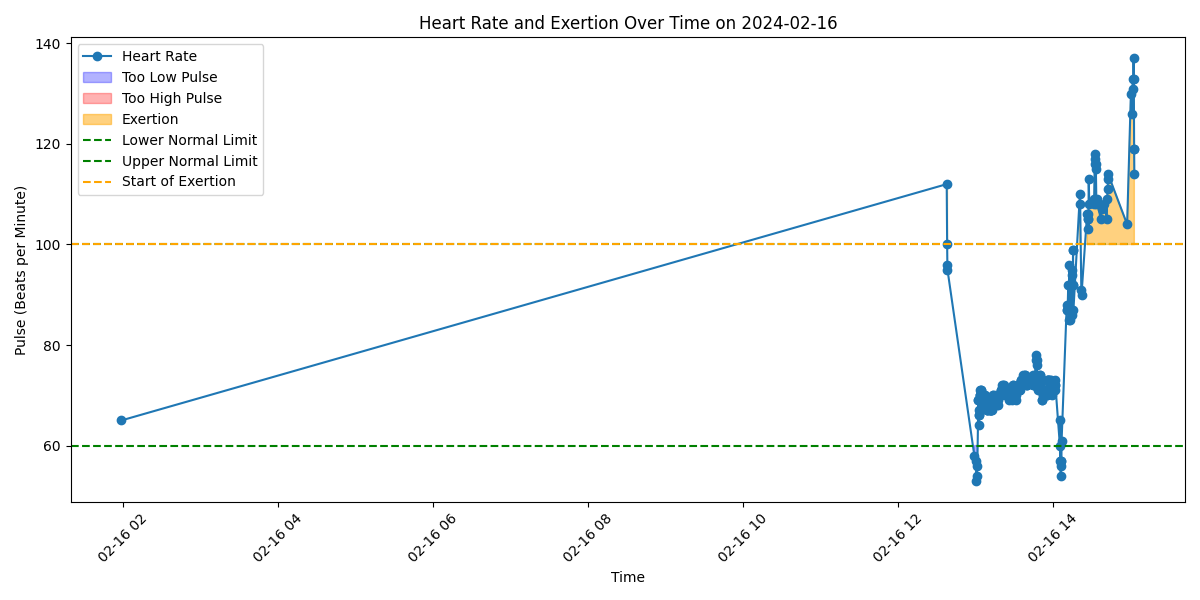
\includegraphics[width=.8\linewidth]{Master Thesis/Plots/heart_rate_plot_2024-02-16.png}
    \caption{}
    \label{fig:test1}
  \end{subfigure}
  \newline
  \begin{subfigure}{.55\textwidth}
    \centering
    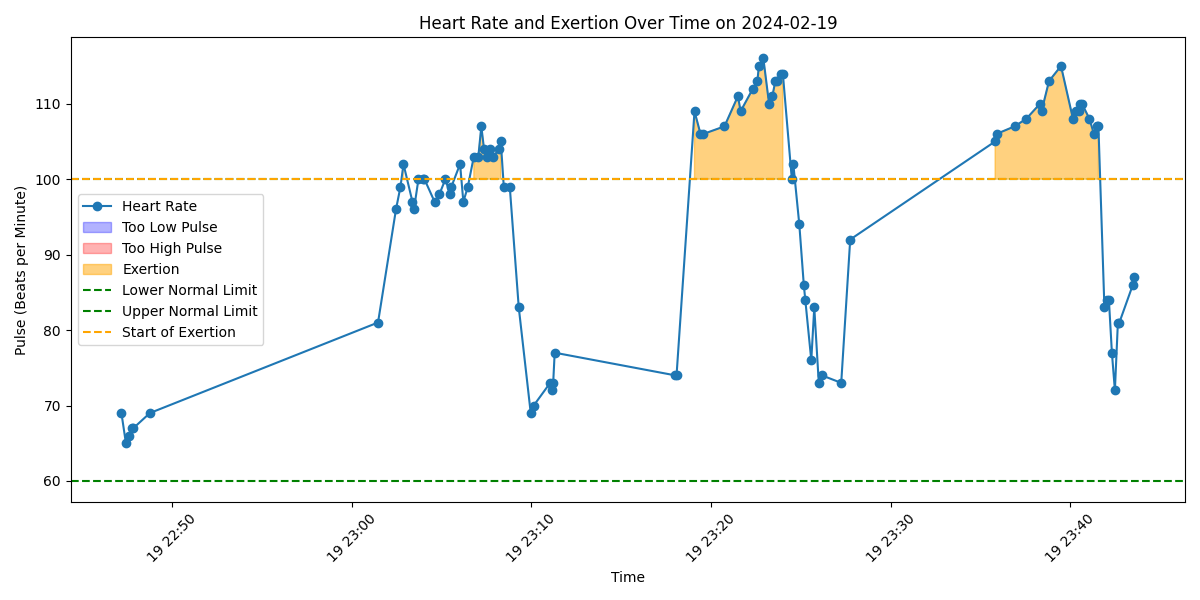
\includegraphics[width=.8\linewidth]{Master Thesis/Plots/heart_rate_plot_2024-02-19.png}
    \caption{}
    \label{fig:test2}
  \end{subfigure}%
  \begin{subfigure}{.55\textwidth}
    \centering
    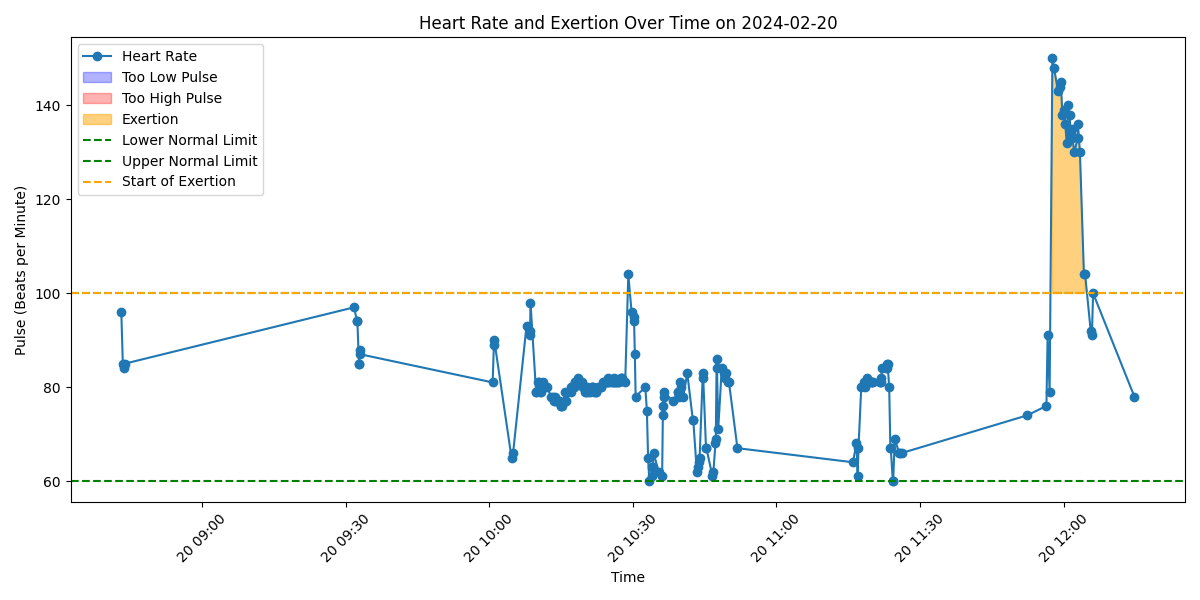
\includegraphics[width=.8\linewidth]{Master Thesis/Plots/heart_rate_plot_2024-02-20.png}
    \caption{}
    \label{fig:test3}
  \end{subfigure}
  \caption{Heart rate data plot to identify the 6MWT interval first part of dataset}
  \label{fig:allintervall6mwt1}
\end{figure}
\FloatBarrier

\FloatBarrier
\begin{figure}[h!]
  \centering
  \begin{subfigure}{.55\textwidth}
    \centering
    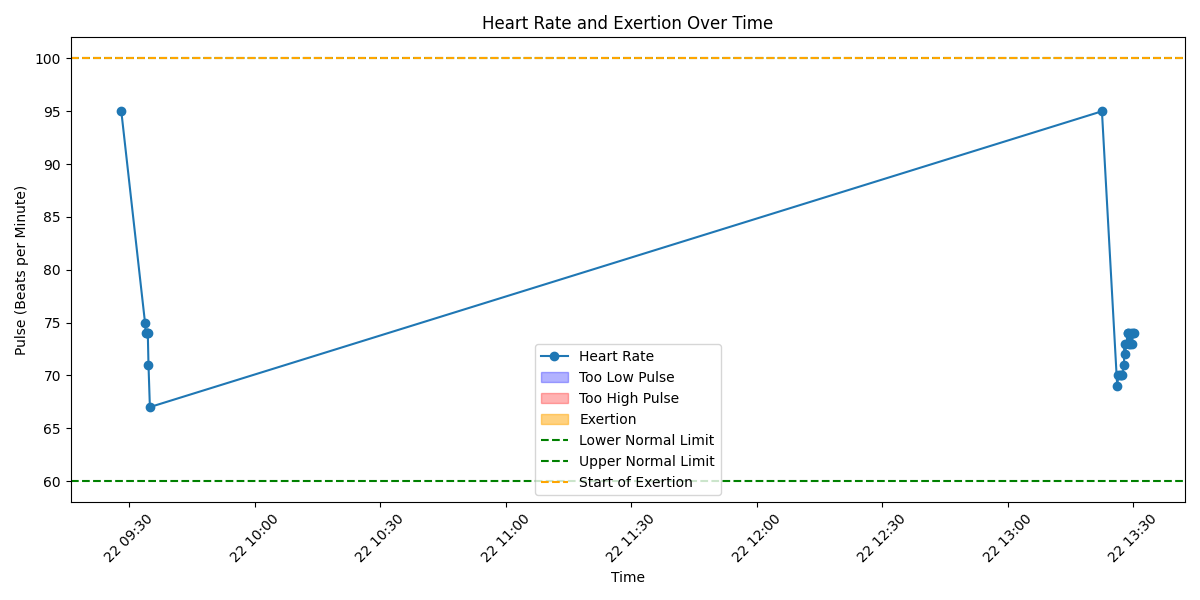
\includegraphics[width=.8\linewidth]{Master Thesis/Plots/6MW_dataset_plot_22_02.png}
    \caption{}
    \label{fig:test4}
  \end{subfigure}%
  \begin{subfigure}{.55\textwidth}
    \centering
    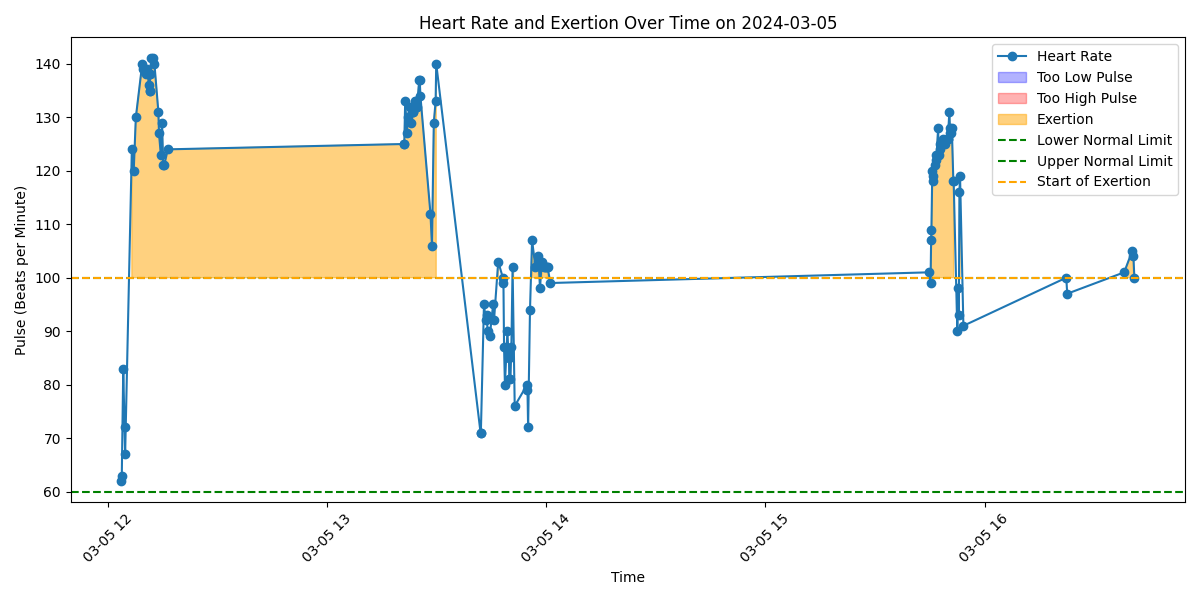
\includegraphics[width=.8\linewidth]{Master Thesis/Plots/heart_rate_plot_2024-03-05.png}
    \caption{}
    \label{fig:test5}
  \end{subfigure}
  \newline
  \begin{subfigure}{.55\textwidth}
    \centering
    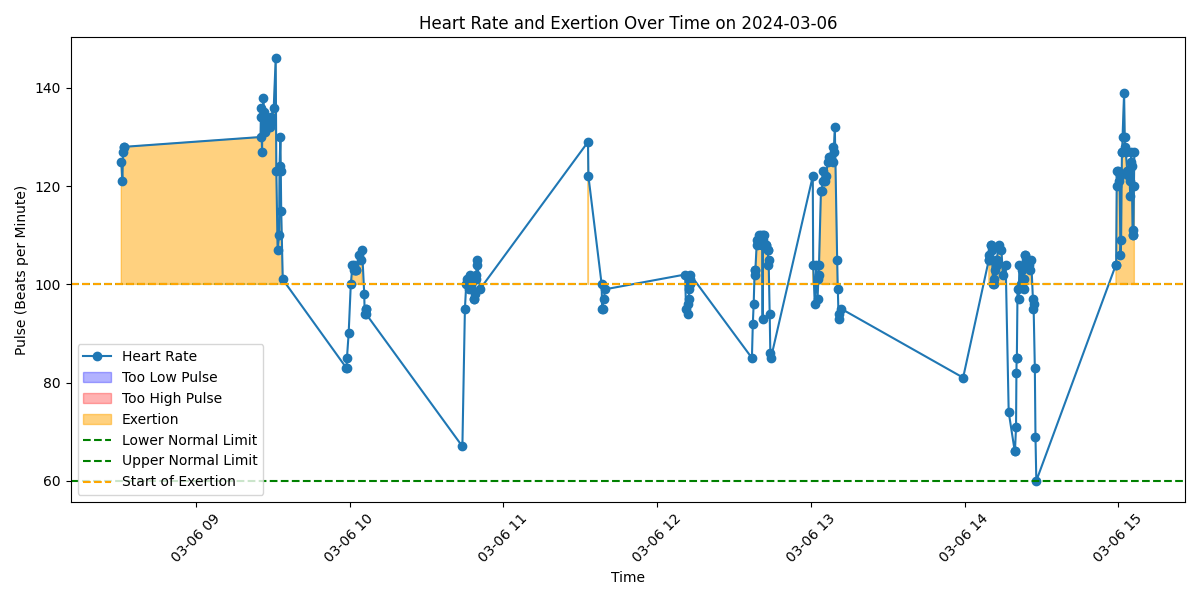
\includegraphics[width=.8\linewidth]{Master Thesis/Plots/heart_rate_plot_2024-03-06.png}
    \caption{}
    \label{fig:test6}
  \end{subfigure}%
  \begin{subfigure}{.55\textwidth}
    \centering
    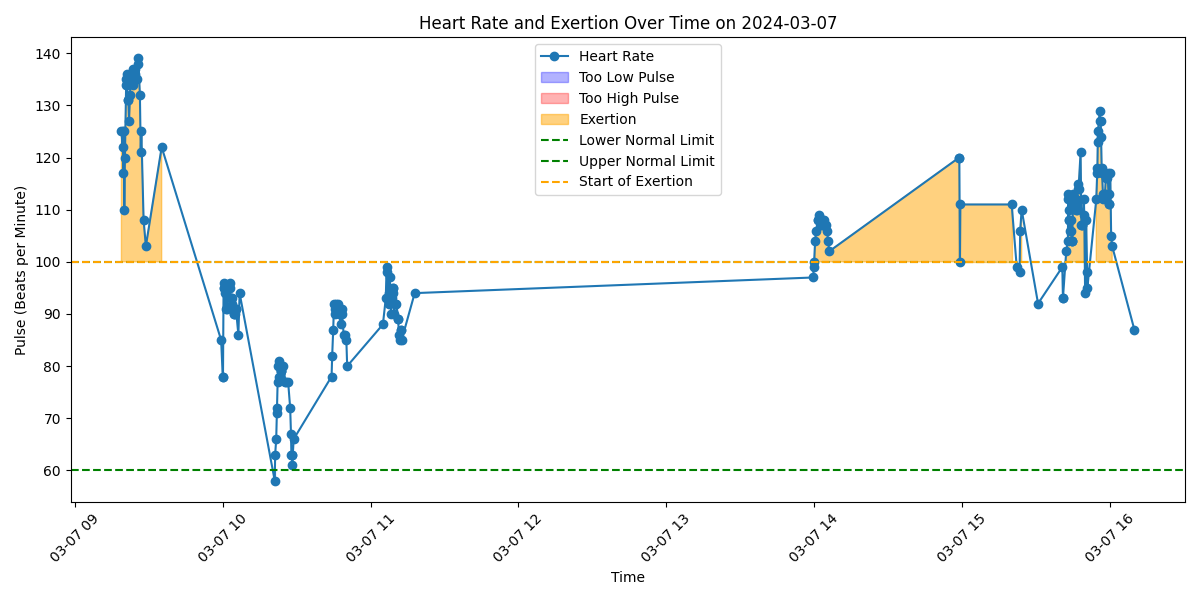
\includegraphics[width=.8\linewidth]{Master Thesis/Plots/heart_rate_plot_2024-03-07.png}
    \caption{}
    \label{fig:test7}
  \end{subfigure}
  \caption{Heart rate data plot to identify the 6MWT interval second part of dataset}
  \label{fig:allintervall6mwt2}
\end{figure}
\FloatBarrier

\FloatBarrier
\begin{figure}[h!]
  \centering
  \begin{subfigure}{.55\textwidth}
    \centering
    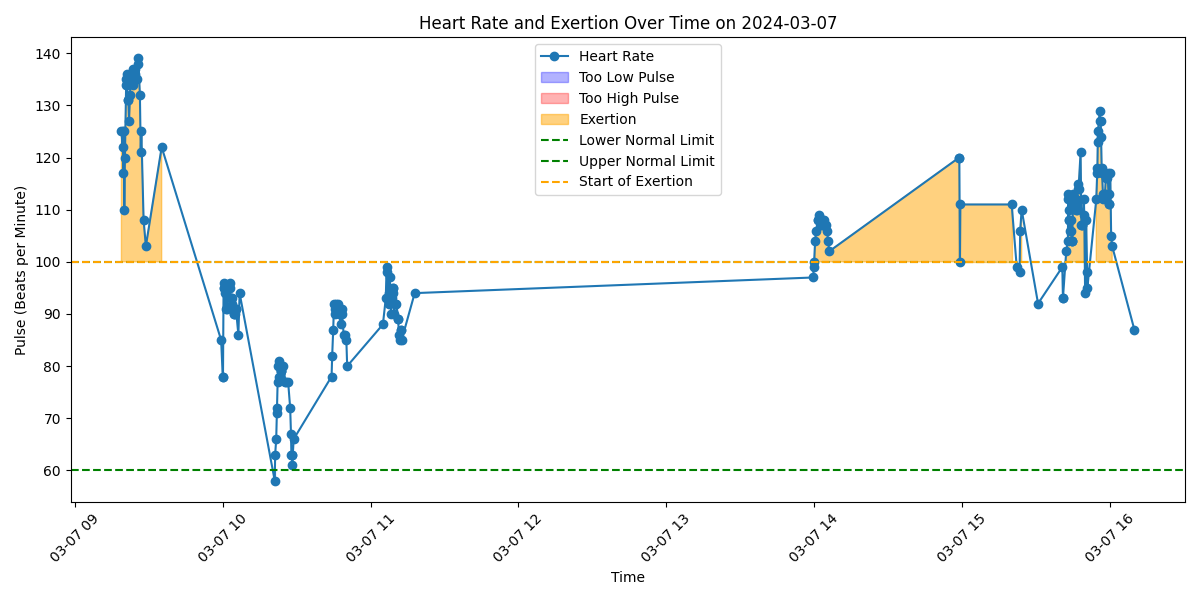
\includegraphics[width=.8\linewidth]{Master Thesis/Plots/heart_rate_plot_2024-03-07.png}
    \caption{}
    \label{fig:test8}
  \end{subfigure}%
  \begin{subfigure}{.55\textwidth}
    \centering
    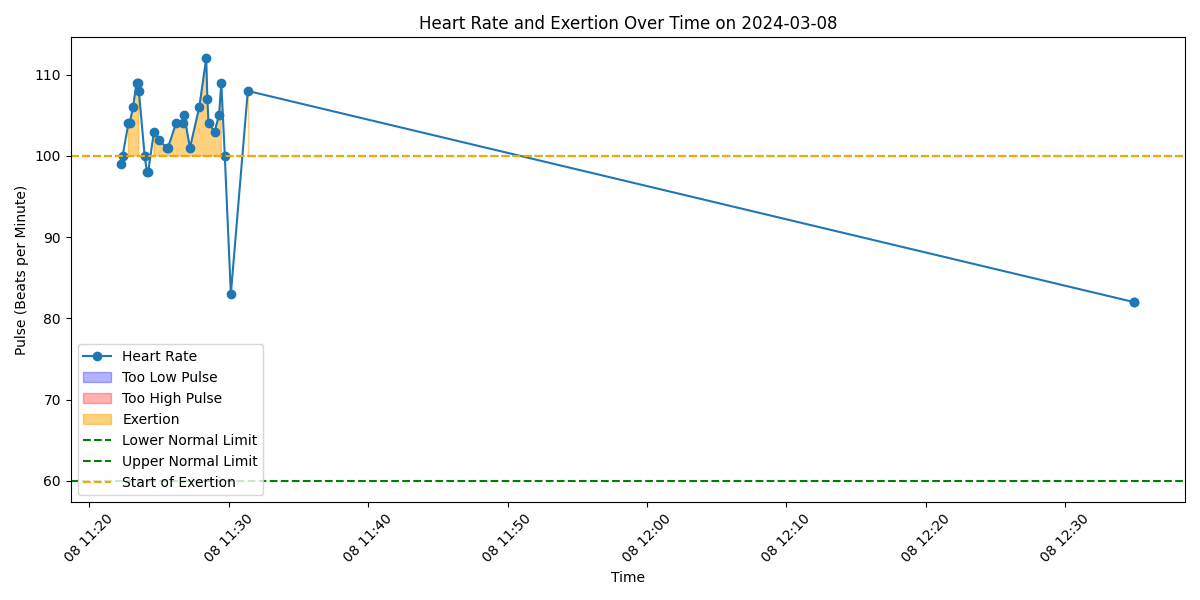
\includegraphics[width=.8\linewidth]{Master Thesis/Plots/heart_rate_plot_2024-03-08.png}
    \caption{}
    \label{fig:test9}
  \end{subfigure}
  \newline
  \begin{subfigure}{.55\textwidth}
    \centering
    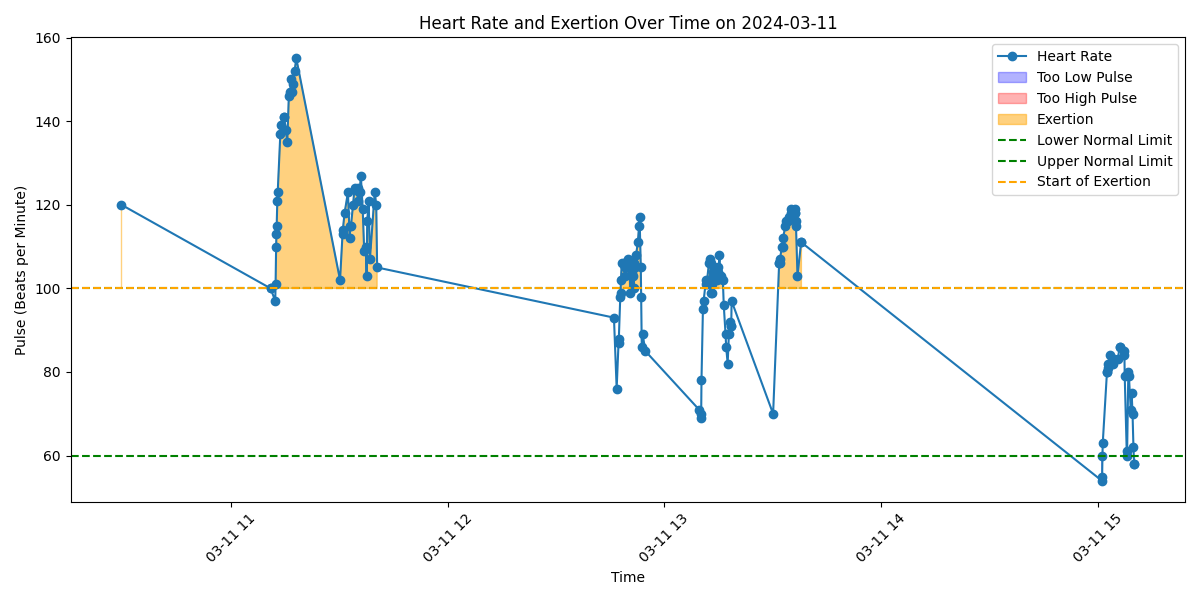
\includegraphics[width=.8\linewidth]{Master Thesis/Plots/heart_rate_plot_2024-03-11.png}
    \caption{}
    \label{fig:test10}
  \end{subfigure}%
  \begin{subfigure}{.55\textwidth}
    \centering
    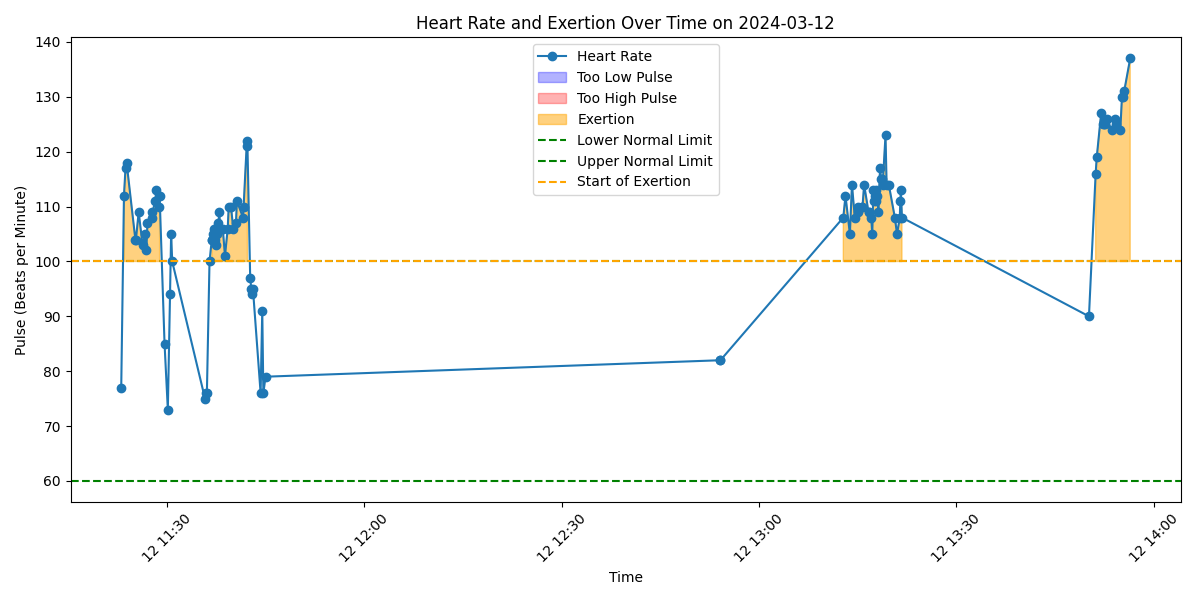
\includegraphics[width=.8\linewidth]{Master Thesis/Plots/heart_rate_plot_2024-03-12.png}
    \caption{}
    \label{fig:test11}
  \end{subfigure}
  \caption{Heart rate data plot to identify the 6MWT interval third part of dataset}
  \label{fig:allintervall6mwt3}
\end{figure}
\FloatBarrier

\FloatBarrier
\begin{figure}[h!]
  \centering
  \begin{subfigure}{.55\textwidth}
    \centering
    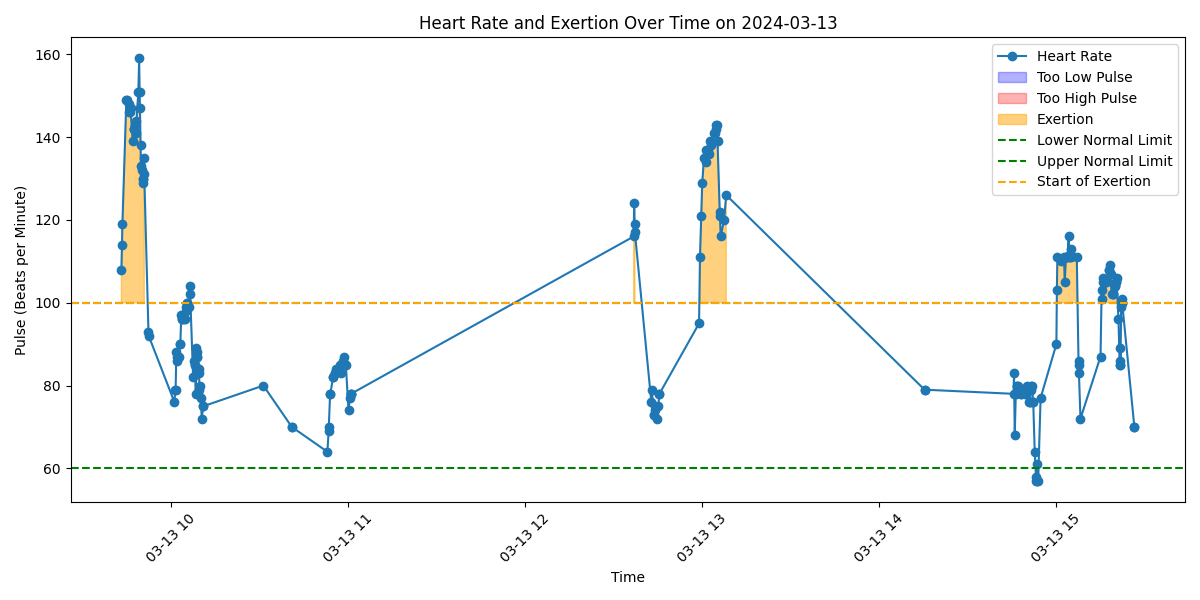
\includegraphics[width=.8\linewidth]{Master Thesis/Plots/heart_rate_plot_2024-03-13.png}
    \caption{}
    \label{fig:test12}
  \end{subfigure}%
  \begin{subfigure}{.55\textwidth}
    \centering
    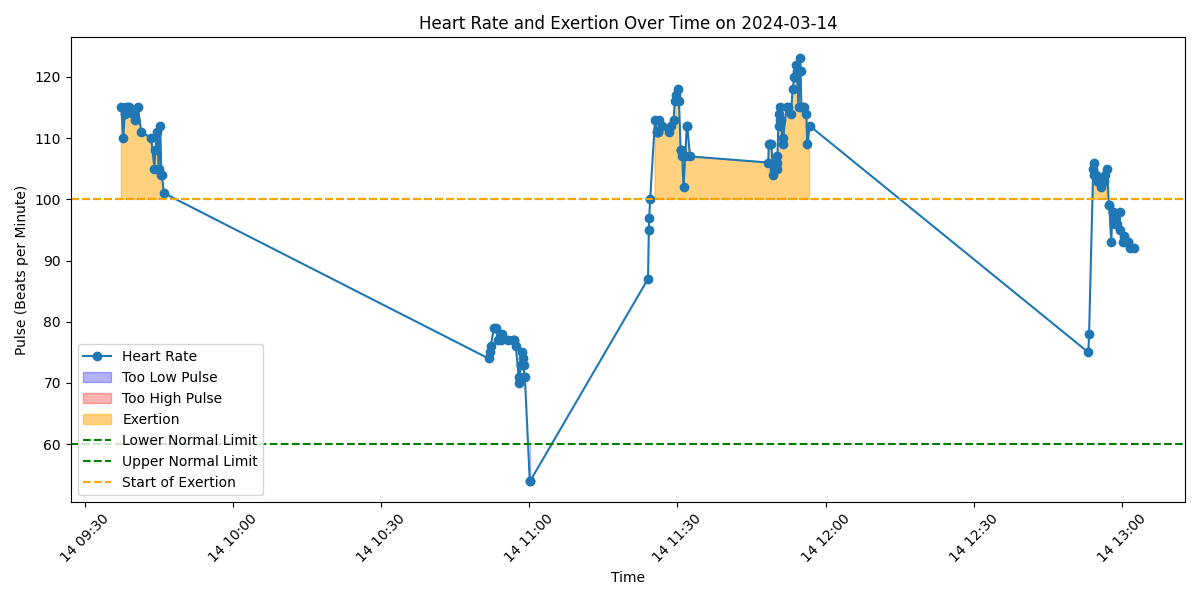
\includegraphics[width=.8\linewidth]{Master Thesis/Plots/heart_rate_plot_2024-03-14.png}
    \caption{}
    \label{fig:test13}
  \end{subfigure}
  \newline
  \begin{subfigure}{.55\textwidth}
    \centering
    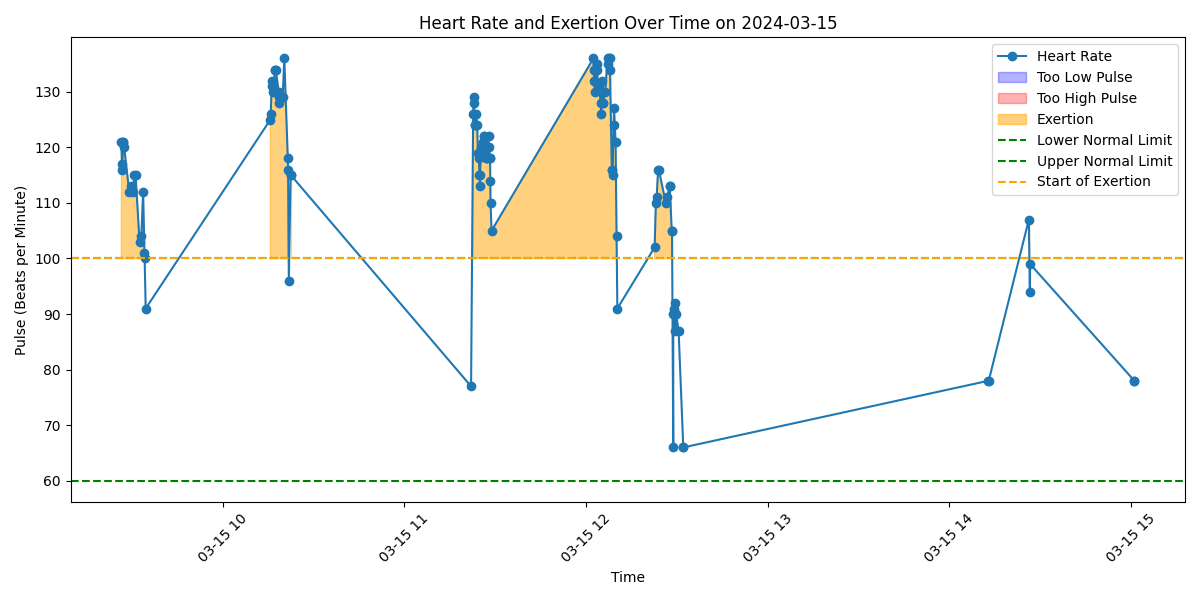
\includegraphics[width=.8\linewidth]{Master Thesis/Plots/heart_rate_plot_2024-03-15.png}
    \caption{}
    \label{fig:test14}
  \end{subfigure}%
  \begin{subfigure}{.55\textwidth}
    \centering
    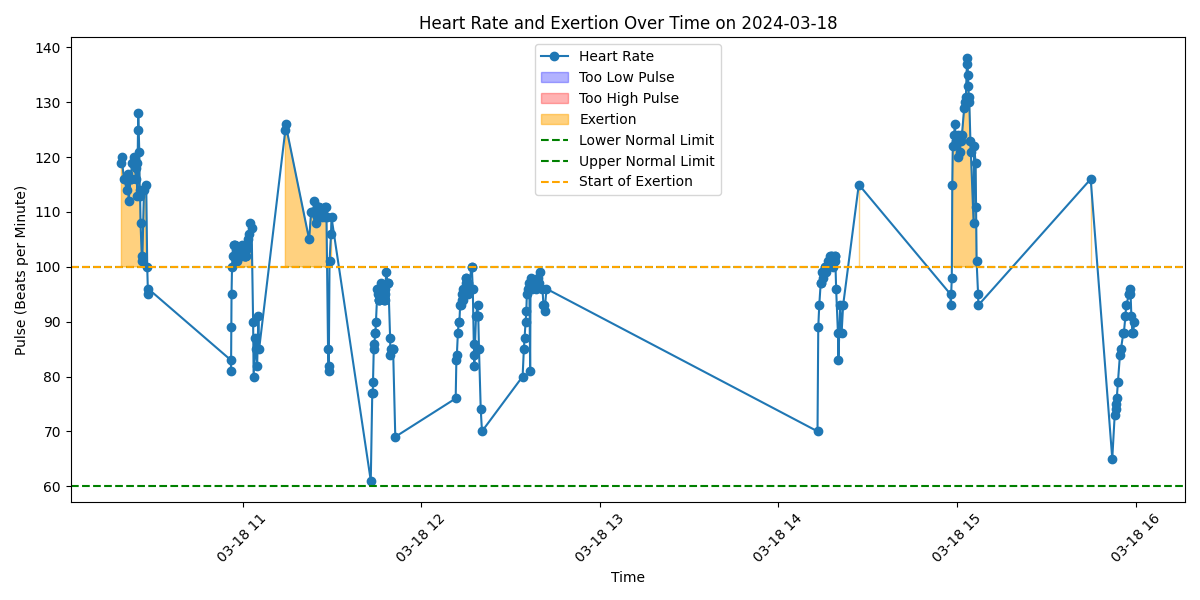
\includegraphics[width=.8\linewidth]{Master Thesis/Plots/heart_rate_plot_2024-03-18.png}
    \caption{}
    \label{fig:test15}
  \end{subfigure}
  \caption{Heart rate data plot to identify the 6MWT interval fourth part of dataset}
  \label{fig:allintervall6mwt4}
\end{figure}
\FloatBarrier

\FloatBarrier
\begin{figure}[h!]
  \centering
  \begin{subfigure}{.55\textwidth}
    \centering
    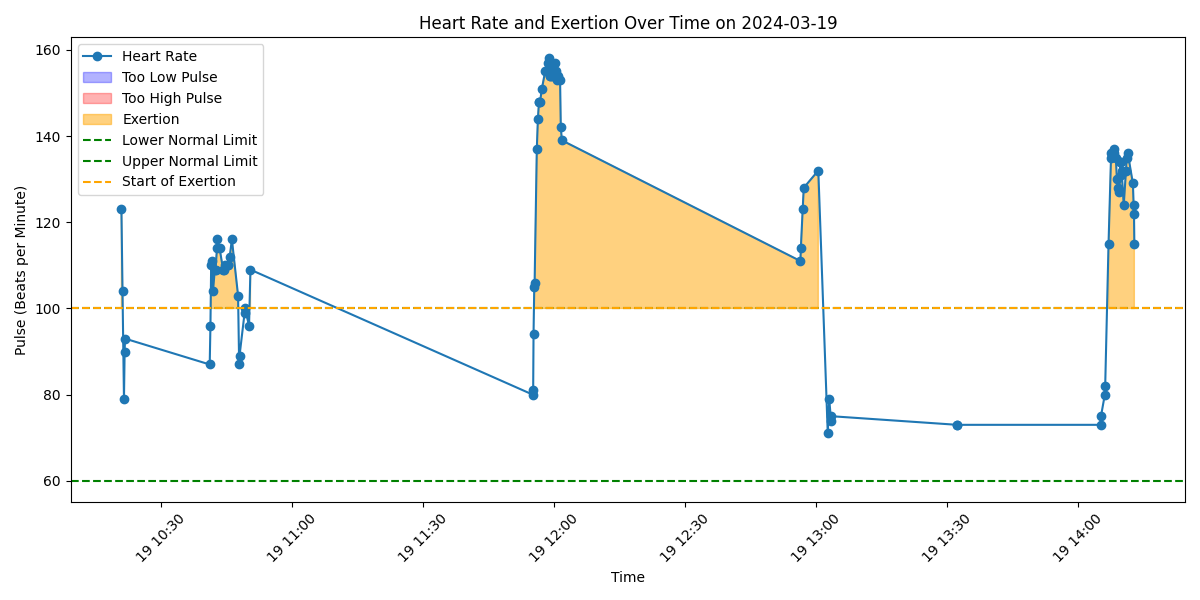
\includegraphics[width=.8\linewidth]{Master Thesis/Plots/heart_rate_plot_2024-03-19.png}
    \caption{}
    \label{fig:test16}
  \end{subfigure}%
  \begin{subfigure}{.55\textwidth}
    \centering
    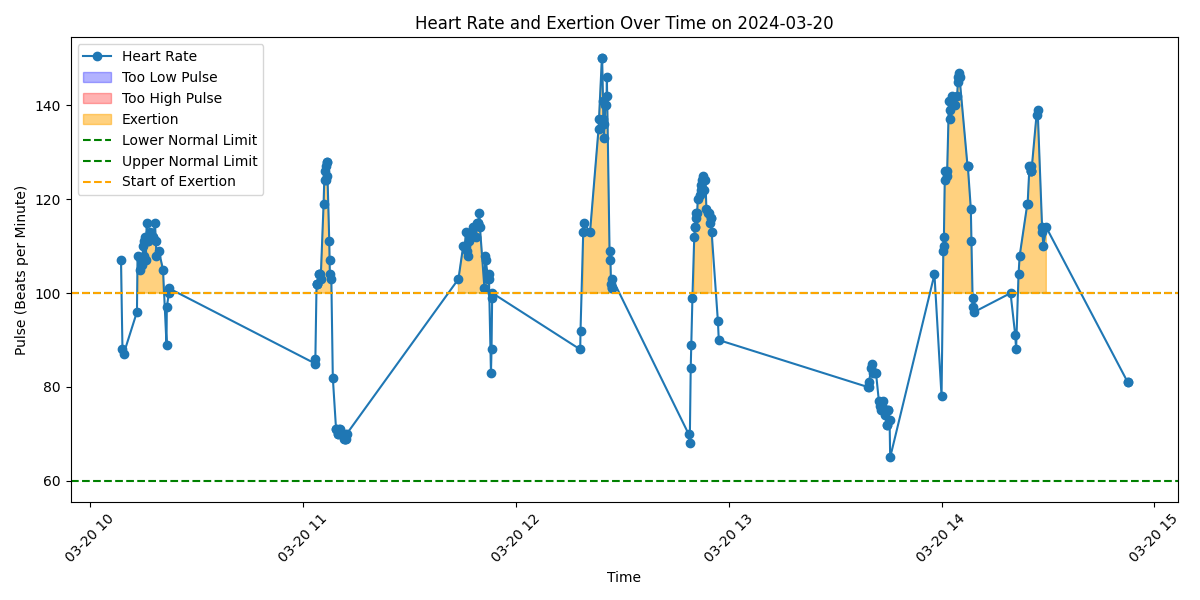
\includegraphics[width=.8\linewidth]{Master Thesis/Plots/heart_rate_plot_2024-03-20.png}
    \caption{}
    \label{fig:test17}
  \end{subfigure}
  \newline
  \begin{subfigure}{.55\textwidth}
    \centering
    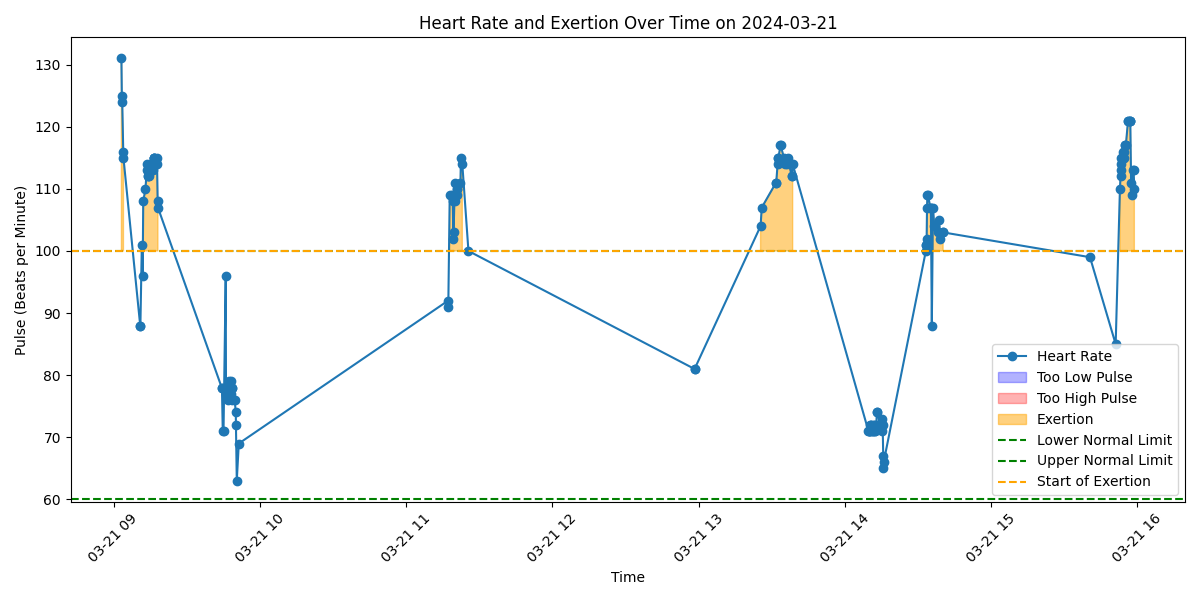
\includegraphics[width=.8\linewidth]{Master Thesis/Plots/heart_rate_plot_2024-03-21.png}
    \caption{}
    \label{ig:test18}
  \end{subfigure}%
  \begin{subfigure}{.55\textwidth}
    \centering
    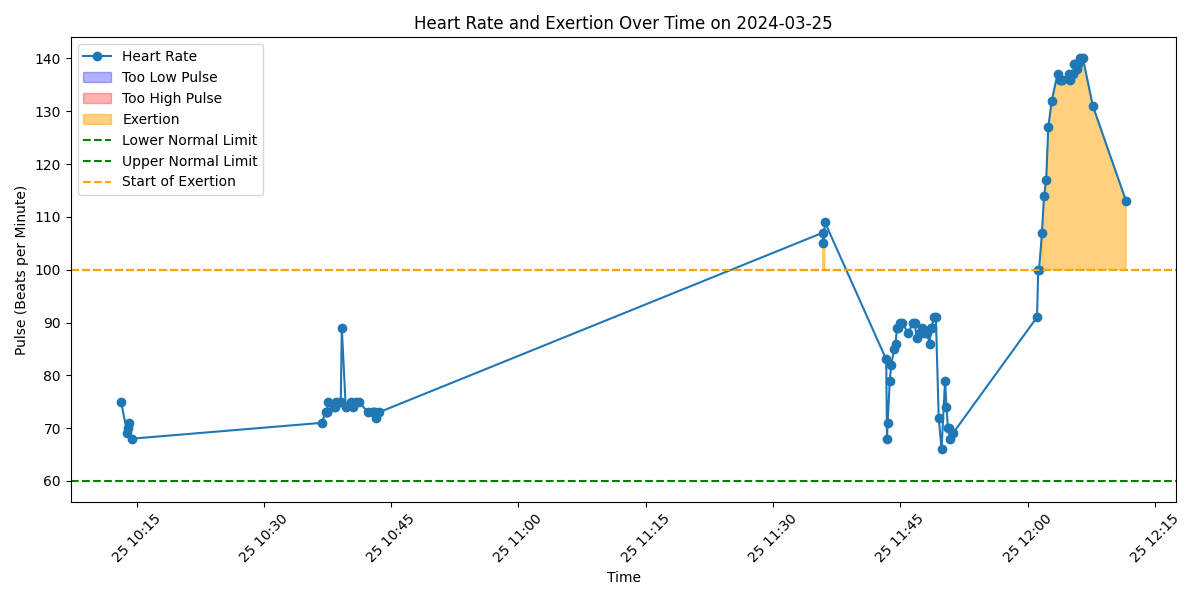
\includegraphics[width=.8\linewidth]{Master Thesis/Plots/heart_rate_plot_2024-03-25.png}
    \caption{}
    \label{fig:test19}
  \end{subfigure}
  \caption{Heart rate data plot to identify the 6MWT interval fifth part of dataset}
  \label{fig:allintervall6mwt5}
\end{figure}
\FloatBarrier

\subsection{Distance Related Data}

After focusing primarily on the course of the heart rate, the focus was shifted. This led to plotting the measured distance from the Apple Watch Ultra per survey week. As seen, two of the five plots can be ignored because they contain only three to five measurement values. Comparing this with the heart rate data for the same interval reveals that these were just technical tests.

In the provided plots, we observe the cumulative distance measured over different weeks.

\FloatBarrier
\begin{figure}[h!]
  \centering
  \begin{subfigure}{.55\textwidth}
    \centering
    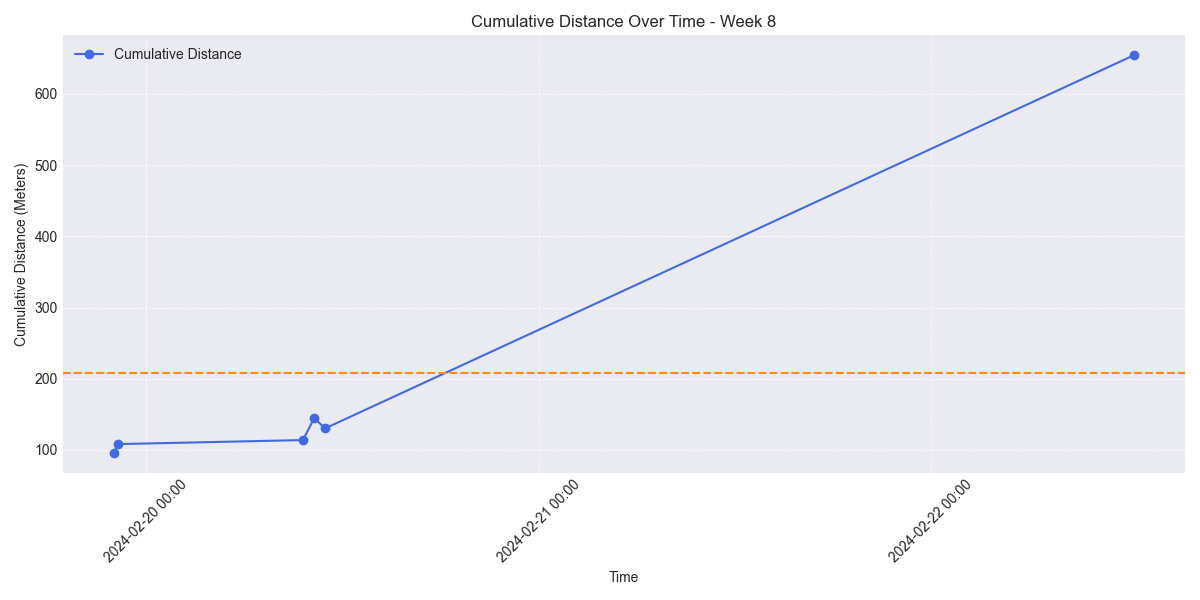
\includegraphics[width=.95\linewidth]{Master Thesis/Plots/cumulative_distance_week_8.png}
    \caption{}
    \label{fig:distrel1}
  \end{subfigure}%
  \begin{subfigure}{.55\textwidth}
    \centering
    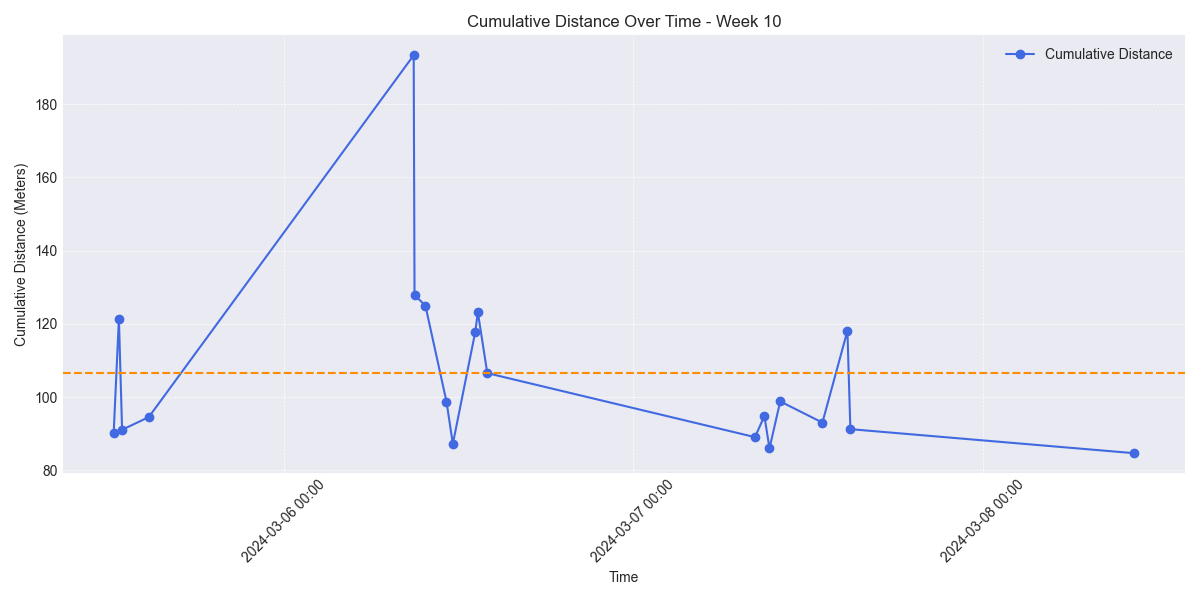
\includegraphics[width=.95\linewidth]{Master Thesis/Plots/cumulative_distance_week_10.png}
    \caption{}
    \label{fig:distrel2}
  \end{subfigure}
  \newline
  \begin{subfigure}{.55\textwidth}
    \centering
    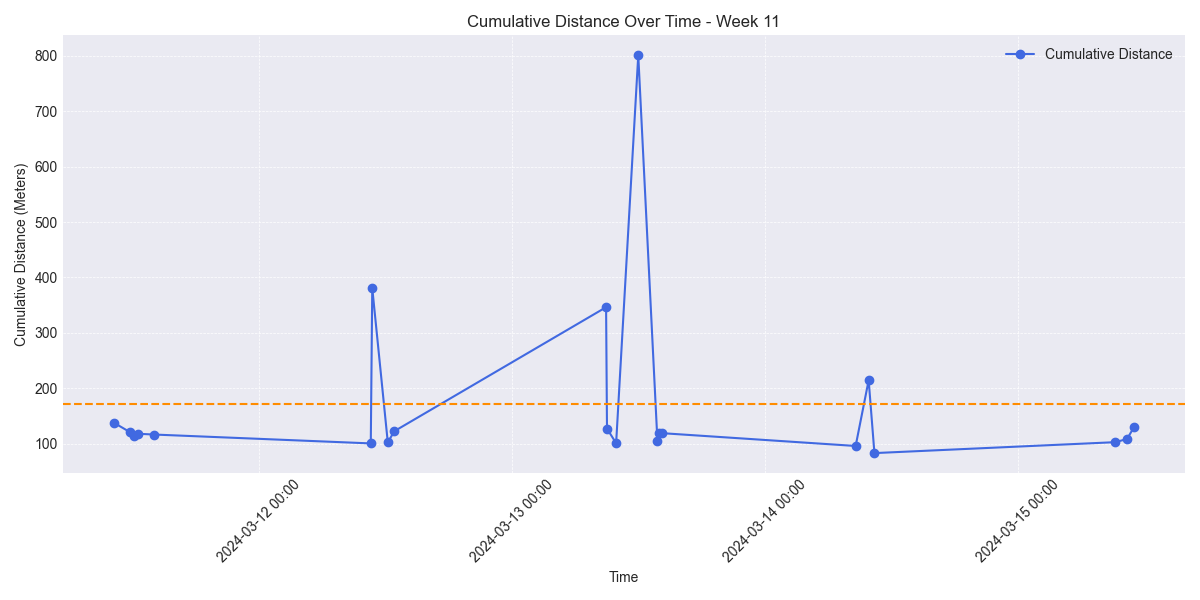
\includegraphics[width=.95\linewidth]{Master Thesis/Plots/cumulative_distance_week_11.png}
    \caption{}
    \label{fig:distrel3}
  \end{subfigure}%
  \caption{Observation of the cumulative distance measured over different weeks first part}
    \label{fig:distcumfirstpart}
\end{figure}
\FloatBarrier

Figure ~\ref{fig:distrel1} shows a steady increase in the cumulative distance over time during the eighth week of the study and data collection, indicating consistent activity throughout the week. The data points are well-distributed, suggesting reliable measurements.

In figure ~\ref{fig:distrel2} we see the cumulative distance fluctuates significantly during the tenth week of data collection, with several peaks and troughs. This irregular pattern could be due to inconsistent activity levels or potential measurement errors during this week.

Figure ~\ref{fig:distrel3} is similar to the tenth week, this plot also shows significant variations in the cumulative distance during the eleventh week of the study. The sharp peaks suggest bursts of activity followed by periods of inactivity. Such patterns might indicate varying levels of physical exertion or possible technical issues.

\FloatBarrier
\begin{figure}[h!]
  \centering
  \begin{subfigure}{.55\textwidth}
    \centering
    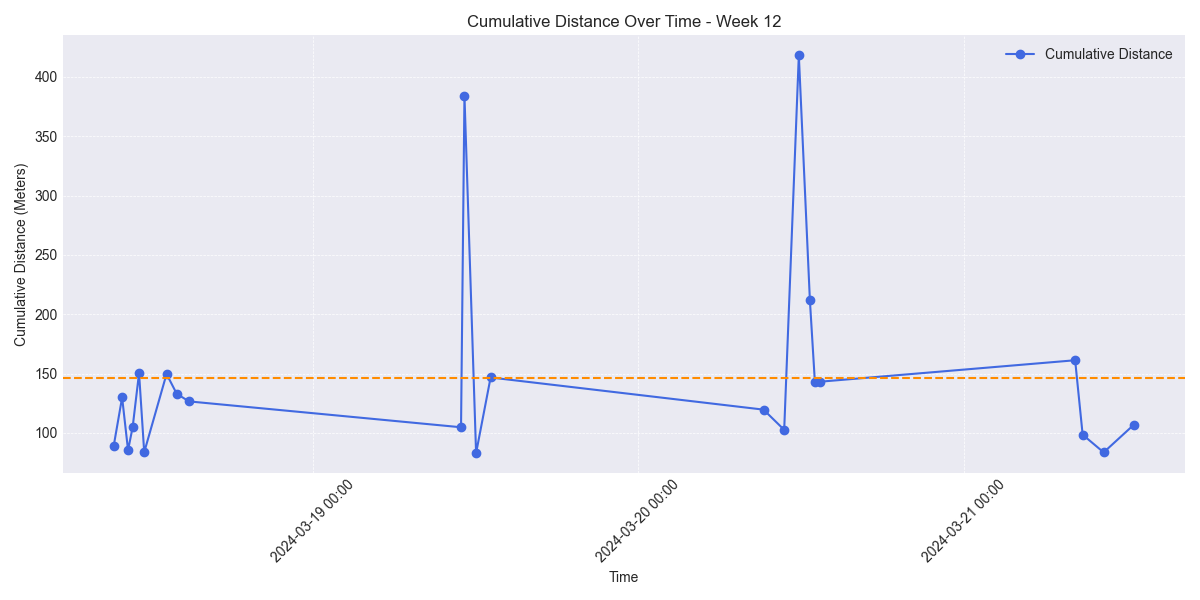
\includegraphics[width=1.0\linewidth]{Master Thesis/Plots/cumulative_distance_week_12.png}
    \caption{}
    \label{fig:distrel4}
  \end{subfigure}%
  \begin{subfigure}{.55\textwidth}
    \centering
    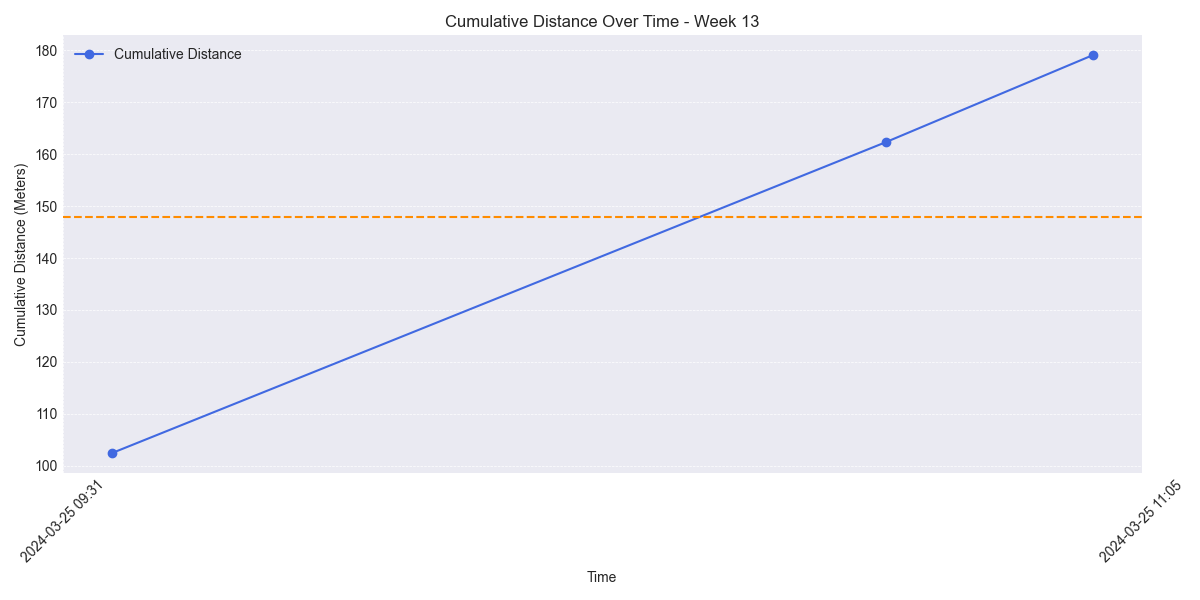
\includegraphics[width=1.0\linewidth]{Master Thesis/Plots/cumulative_distance_week_13.png}
    \caption{}
    \label{fig:distrel5}
  \end{subfigure}
  \caption{Observation of the cumulative distance measured over different weeks second part}
    \label{fig:distcumsecondpart}
\end{figure}
\FloatBarrier

Figure ~\ref{fig:distrel4} displays several spikes in the cumulative distance during the twelfth week, similar to Week eleven. However, the overall trend appears to be more stable towards the end of the week. This could imply an initial phase of irregular activity followed by more consistent measurements.

Figure ~\ref{fig:distrel5} shows a linear increase in cumulative distance in week 13, indicating a consistent level of activity throughout the week. The steady upward trend suggests reliable and continuous measurements without significant fluctuations.

\newpage
\subsection{Correlation Between Weight, Height and Sex}

In the initial stages of this study, the sex of the subjects was not available. To infer the sex from the dataset, an analysis based on the height and weight of the subjects was performed. The dataset was divided into intervals for both height and weight to approximate sex prediction. In the following plot, two lines represent approximate height and weight, respectively. These lines are further divided into male and female categories, resulting in a total of four lines.

\FloatBarrier
\begin{figure}[h!]
\centering
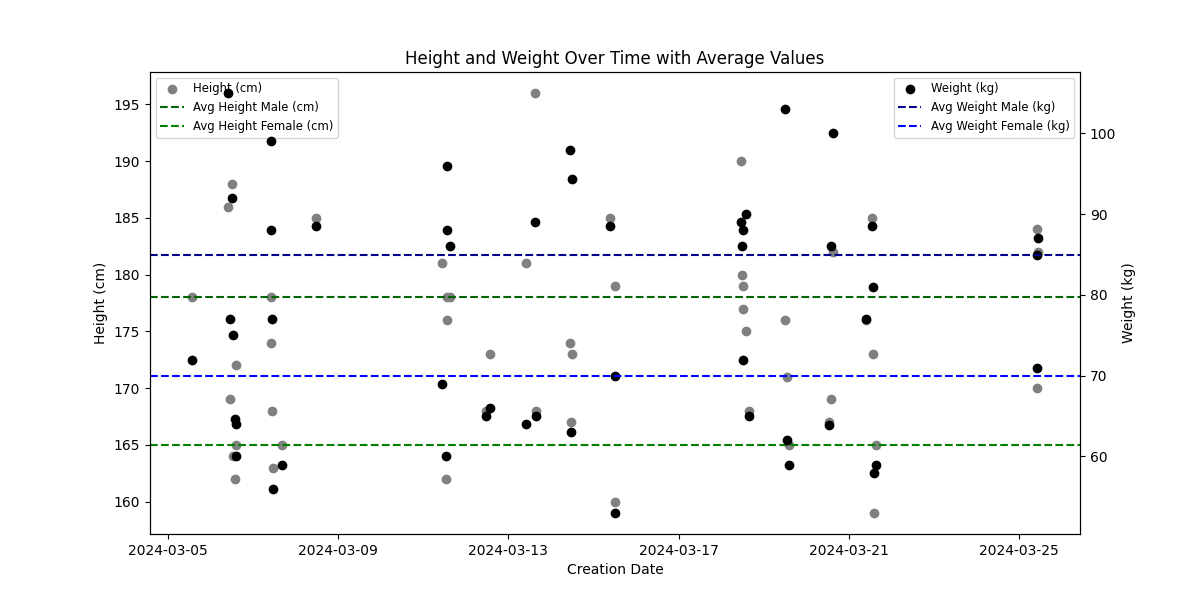
\includegraphics[width=1.0\linewidth]{Master Thesis/Plots/weights&hights.png}
\caption{Height and Weight Correlation of sex}
\label{fig:weightheightcorrsex}
\end{figure}
\FloatBarrier







